% this is a comment in latex
% substitute this documentclass definition for uncommented one
% to switch between single and double column mode
\documentclass[11pt,twocolumn]{article}
%\documentclass[11pt]{article}

\usepackage{fullpage}
\usepackage{subfigure,indentfirst}
% for url
\usepackage{hyperref}
% for underlined text
\usepackage[normalem]{ulem}
% for including pdf figures
\usepackage{graphicx}
\usepackage{amsmath}

% my own versions: my_enumerate and my_itemize
\newenvironment{my_enumerate}{
  \begin{enumerate}
    \setlength{\itemsep}{1pt}
      \setlength{\parskip}{0pt}
\setlength{\parsep}{0pt}}{\end{enumerate}
}

\newenvironment{my_itemize}{
  \begin{itemize}
    \setlength{\itemsep}{1pt}
      \setlength{\parskip}{0pt}
\setlength{\parsep}{0pt}}{\end{itemize}
}

% this starts the document
\begin{document}

\title{CS87 Project Report: Trade-offs when Factoring Large Numbers in Parallel with MPI}

\author{Tarang Saluja, Tai Thongthai\\
Computer Science Department, Swarthmore College, Swarthmore, PA  19081}

\maketitle


\begin{abstract}
RSA (Rivest-Shavir-Adleman) is a public-key, asymmetric cryptosystem which is commonly used to protect and transmit data. After a public key is used to encrypt the data, the recipient can use a private key to decrypt the encrypted data. To decrypt an RSA encryption without access to the private key, one must factor the public key, which is a large number $N$ that is the product of two large primes, in a feasible amount of time. This is a difficult problem to do with brute force, and a variety of algorithms have been developed to factor $N$ more quickly. One of these algorithms is called the \textit{Quadratic Sieve}, and most of the time is spent in the \textit{sieving step}. During the \textit{sieving step}, we repeatedly divide a large amount of numbers by increasingly large primes until enough of them are fully factored. As such, it is most useful to parallelize the sieving step. We compare the speeds of two MPI Boss-Worker paradigm parallelizations of the sieving step which trade off on less communication and flexibility of contribution from workers. Testing our two different MPI parallelizations and our sequential implementation reveals that the MPI strategy which has increased communication but allows some workers to contribute more than others has equal or slightly better performance when there are a higher number of worker processes (usually greater than 8 or 16) and worse performance when there are less processes, given a large enough key size. Furthermore, parallelization yields significant speedup.
\end{abstract}


\section {Introduction}
\indent Since the RSA cryptosystem can be cracked by factoring a large $N$ which is the product of two large primes, we attempt to see how parallelization can be used to achieve this factorization faster. With this kind of experiment, we can make determinations about the security of RSA encryption against small-scale bad actors and learn more about what kind of parallelization is more likely to be used. For instance, if we find that our first parallelization is a lot faster and works well against the standard keys that we are using, perhaps specific keys which take longer with the first parallelization should be used. By implementing two different parallelizations, one which involves constant communication between the boss process and worker processes, and another in which the boss process only takes from the worker processes, we ran tests and found that when more flexibility of contribution is enabled by more communication, we see better performance when there are more processes, given a large enough key size. However, less flexibility of contribution and less communication performs better when there are less processes.

\subsection{Introduction to RSA}
\indent RSA is an asymmetric, public key cryptosystem that is widely used to encrypt and protect small pieces of data. Let Alice and Bob be the players using the RSA cryptosystem. As an asymmetric cryptosystem, Alice has both the public key and the private key, while Bob has only the public key. Now Bob can use the corresponding encryption function $e : \mathcal{M} \to \mathcal{C}$ to encrypt the message and send $e(m)$. As Alice has the private key, she can use the corresponding decryption function $d: \mathcal{C} \to \mathcal{M}$ to decrypt the message, as the private and public keys are chosen to ensure $d(e(m)) = m$. \\
\indent For RSA encryption which uses large prime numbers, the public key is the set $\{N, e \}$, where $N = pq$ for two large prime numbers $p, q$ and $e < \varphi(N) = (p-1)(q-1)$. The private key is some $d$ such that $ed \equiv 1 \pmod{\varphi(N)}$. An eavesdropper who can see the public key $\{N, e \}$ and the message which is sent, which is $e(m)$, must know $d$ to decrypt the message. To find $d$ in a feasible amount of time, they must know $\varphi(N) = (p-1)(q-1)$, which involves factoring $N$ into $pq$ \cite{hoffstein:cryptography}.

\subsection{Introduction to Quadratic Sieving}
Since it is difficult to factor large $N$, RSA is a relatively secure cryptosystem \cite{hoffstein:cryptography}. However, heightened computing power, negligence, and creative attack algorithms make it possible to attack RSA encryption \cite{lifchitz:rsa_break}. We are interested in using ideas from parallel and distributed computing to further optimize the Quadratic Sieve attack method. As outlined in A Tale of Two Sieves \cite{pomerance:tts}, the Quadratic Sieve method has the following steps:

\begin{enumerate}
    \item Generate a Factor Base. This involves creating a set of primes.
    \item Sieving. First, we evaluate $Q(x) = x^2 - N$ for a large number $x > \lfloor \sqrt{N} \rfloor + 1$ to ensure that $Q(x) > 0$. Then we use only primes from the factor base to find as many factorizations $Q(x) = \displaystyle \prod_{i = 1}^n p_i^{e_i}$ as possible.
    \item Find equations of the form $X^2 \equiv P^2 \pmod{N}$. This entails finding some subset of $x$ evaluated at the polynomial such that such that $\left( \displaystyle \prod_{x \in S} x \right)^2 = p_1^{2e_1} p_2^{2e_2} \ldots p_n^{2e_n} \pmod{N}$, and is often found with linear algebra. Here $S \subseteq \{x_1, x_2 \ldots x_m \}$ \cite{landquist:qs}.
\end{enumerate}

\indent As an example, suppose that $N = 527$. After we generate a factor base, we can factor $Q(x) = x^2 - 527$ for $x = 23, 24, 25, ...$. As we factor these polynomial evaluations, we find equations of the form $x_k^2 - 527 \equiv \displaystyle \prod_{i = 1}^n p_i^{e_i}$, which means that $x_k^2 \equiv \displaystyle \prod_{i = 1}^n p_i^{e_i} \pmod{527}$. We can see then for instance that $23^2 \equiv 2 \pmod{527}, 24^2 \equiv 7^2 \pmod{527}, 25^2 \equiv 2 \cdot 7^2 \pmod{527}$ and so on. \\
The quadratic sieve's key idea is to identify an equation of the form $x^2 \equiv y^2 \pmod{N}$, and in this case we find quite quickly that $24^2 \equiv 7^2 \pmod{527}$. This helps us because $x^2 \equiv y^2 \pmod{N} \iff (x+y)(x-y) \equiv 0 \pmod{N}$ by the formula for the difference of squares.  In other words, $(x+y)(x-y) = kN$ for some $k \in \mathbf{N}$. As long as we don't have $x+y = k$ or $x-y = k$, it follows that $x-y$ or $x+y$ and $N$ will share some factor \cite{hoffstein:cryptography}. Hence, we compute  $\gcd(x+y, N)$ or $\gcd(x- y, N)$, something which can be accomplished in a computationally feasible amount of time with Euclid's Algorithm. In the case of our example we see $(24 + 7)(24 - 7) \equiv 0 \pmod{527}$, and indeed $\gcd(31, 527) = 31$ is a factor.

\indent While it is true that $N = pq$ for $p, q > 2$ can always be expressed as the difference of perfect squares $N = \left( \frac{p+q}{2} \right)^2 - \left( \frac{p-q}{2} \right)^2$, it is quite difficult to find these values when $N$ is huge. Thus, we take the different approach of combining relations. For example, our relations above show us that $23^2 \cdot 25^2 \equiv 2^2 \cdot 7^2 \pmod{527}$, giving us that $(575 + 14)(575 - 14) \equiv 0 \pmod{527}$. Then computing $\gcd(589, 527) = 31$.

\indent Such a combination of relations are much harder, if even possible, to notice with far larger numbers. Suppose that $x_k^2 - 527 = \displaystyle \prod_{i = 1}^n p_i^{e_{i, k}}$, where $e_{i, k}$ is the exponent of $p_i$ in the factorization of $x_k$. Then we must find some $S \subset \{x_1, x_2, \ldots x_m \}$, where these are the $x$ at which we evaluated $Q(x)$, such that both sides in the congruence

$$\displaystyle \prod_{x_k \in S} x_k^2 \equiv  \displaystyle \prod_{i = 1}^n p_i^{\displaystyle \sum_{x_k \in S} e_{i, k}} \pmod{527}$$

are perfect squares. The latter is a perfect square only if $\displaystyle \sum_{x_k \in S} e_{i, k} \equiv 0 \pmod{2}$ for all $i$. Now note that $\displaystyle \sum_{x_k \in S} e_{i, k} = \displaystyle \sum_{k = 1}^m e_{i, k} I(x_k)$, such that $I(x_k) = 1$ if $x_k \in S$ and $I(x_k) = 0$ if $x_k \not \in S$. Thus, we are really trying to solve the system of equations:

$$\displaystyle \sum_{k = 1}^m e_{1, k} I(x_k) \equiv 0 \pmod{2}$$
$$\displaystyle \sum_{k = 1}^m e_{2, k} I(x_k) \equiv 0 \pmod{2}$$
$$\vdots$$
$$\displaystyle \sum_{k = 1}^m e_{n, k} I(x_k) \equiv 0 \pmod{2}.$$

We can write this as a matrix equation $\mathbf{AX} = \mathbf{B}$, where

$A = \begin{pmatrix}
e_{1, 1} & e_{1, 2} & e_{1, 3} & \cdots & e_{1, m} \\
e_{2, 1} & e_{2, 2} & \cdots & & \\
e_{3, 1} & \vdots & \ddots & & \vdots\\
\vdots & & & & \\
e_{n, 1} & & \cdots & & e_{n, m}
\end{pmatrix}$

such that $A_{i, j} = e_{i, j}$, where $i$ denotes that it is the exponent for $p_i$ and $j$ denotes that it is for the factorization of $Q(x_j)$, and $\mathbf{X}$ is a column vector with $I(x_1), I(x_2) \ldots I(x_m)$ such that $X \in \mathbf{R}^m$ and $\mathbf{B}$ is a column vector of zeroes such that $\mathbf{B} \in \mathbf{R}^n$. If we solve this modulo $2$, which means that we solve in the field $GF(2)$, which is the general field with characteristic 2, we should find values for $I(x_1), I(x_2) \ldots I(x_n)$ which indicate inclusion or exclusion of the given $x_k$ from $S$.

\indent Since an odd value in $A$ contributes as much as $1$ to the parity of the result and an even value in $A$ contributes as much as $0$ to the parity of the result, we can replace all values in the matrix $A$ with 0 and 1 bits which correspond to parity. Then all of the elements in $\mathbf{A}$ and $\mathbf{B}$ are in $GF(2)$, and we can solve for $\mathbf{X}$ like any linear system of equations over $GF(2)$. Once we find for which $x_k$, we have $I(x_k) = 1$, we will have the equation

$$\displaystyle \prod_{k \in S} x_k^2 \equiv  \displaystyle \prod_{i = 1}^n p_i^{\displaystyle \sum_{k \in S} e_{i, k}} \pmod{527}$$

such that both sides are perfect squares, and hence we can finish the computation \cite{landquist:qs}.

\indent As each solution has roughly a 50 \% chance of success when we take $\gcd(x - y, N)$ or $\gcd(x + y, N)$ \cite{asbrink:parallelqs}, finding $n$ solutions yields a $1 - \frac{1}{2^n}$ probability of success. As such, we take the suggestion from the implementation published on a website called Bytopia to find $10$ more relations than the amount of prime numbers \cite{bytopia:help}. That gives us a $\frac{1023}{1024}$ probability of success. Once the primes $p$ and $q$ are found, the person who wants to break RSA can quickly find some $d$ such that $ed \equiv 1 \pmod{(p-1)(q-1)}$, which once again is solved "fast" by the Euclidean algorithm, an extremely important polynomial time algorithm in Number Theory which is constantly improved due to its applicability \cite{collins:euclid}.


\subsection{Solution and Parallelization}
Many solutions of the Quadratic Sieve and it's variations, such as the Multiple Polynomial Quadratic Sieve (MPQS) which factors evaluations at multiple polynomials, first create a sieving interval of a fixed size and then perform the sieving process on it \cite{bytopia:help}. Recall that the sieving interval is the set created by evaluating a polynomial, or multiple polynomials in the case of MPQS. The sieving process involves iterating through the primes in the factor base and dividing the numbers in the sieving interval by a given prime when applicable. This continues until we know the factorization for enough numbers in the interval.

\begin{figure}[!htb]
    \centering
   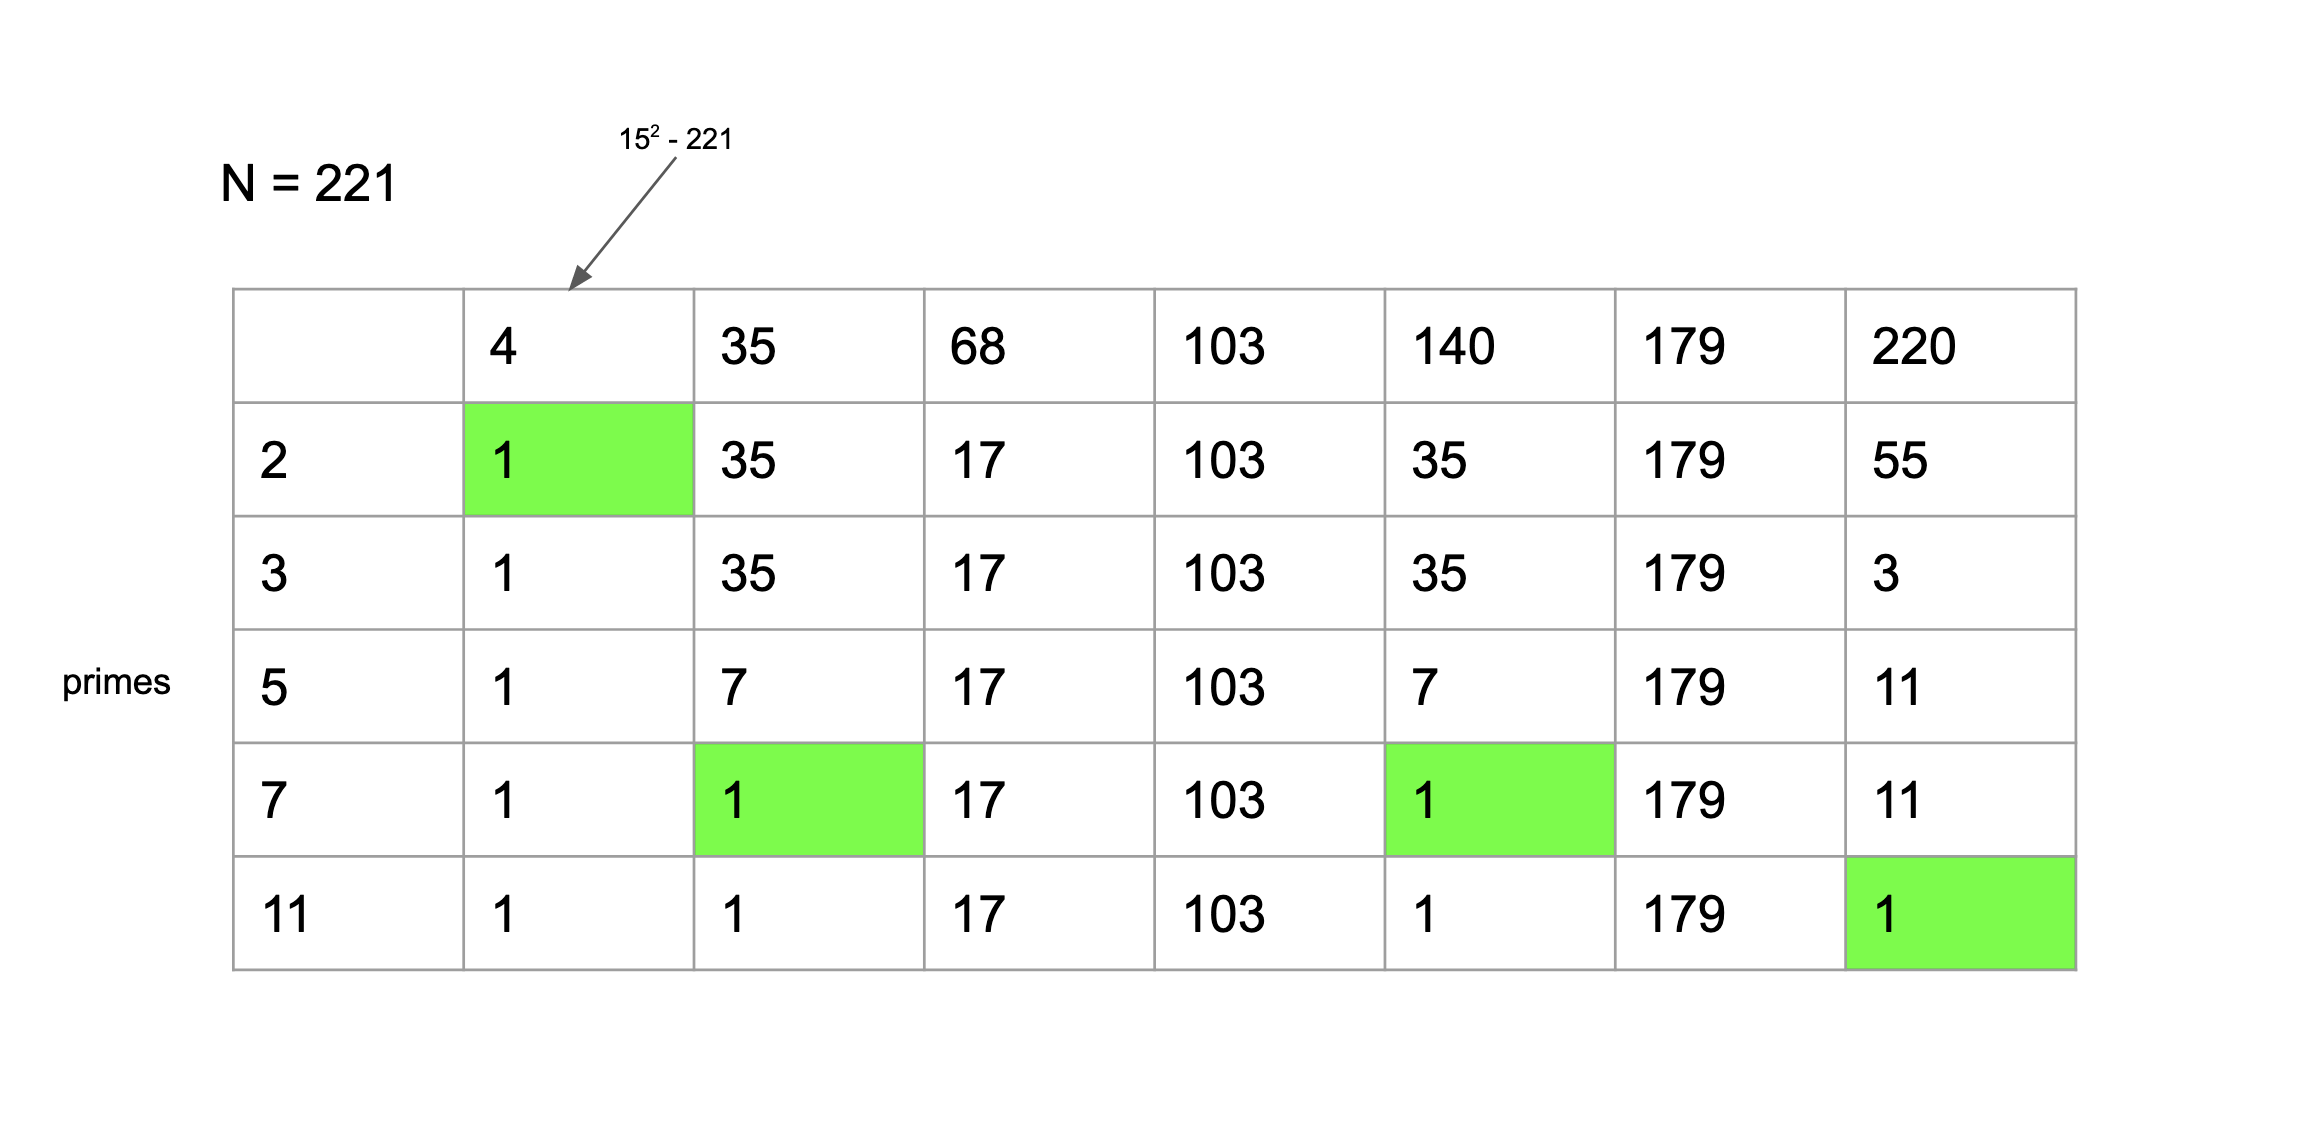
\includegraphics[scale = 0.2]{QS1.png}
    \caption{For each prime, we update each number in the column by dividing it with a given prime as many times as possible}
    \label{QS-Samp}
\end{figure}



Figure 1 depicts what our sieving step looks like, and we shade the boxes where we have enough information to determine a relation. However, this was challenging to implement in our case because of memory constraints. While other implementations can have a smaller sieving interval because they use multiple polynomials to find relations, we decided to work with the single polynomial quadratic sieve \cite{silverman:mpqs}. Furthermore, others may have systems with more space. As the author of the Bytopia implementation notes, it is possible to implement Quadratic Sieve without a sieving interval \cite{bytopia:help}. In particular, one can evaluate the polynomial at a value, sieve just that polynomial, and then save it and the factorization if applicable. While this is a feasible sequential implementation in which we just change the order of our operation by iterating through polynomial evaluations and seeing if we can factorize them instead of iterating through primes and seeing which polynomial evaluations can be factorized, this is not very feasible to parallelize. In particular, if we tried to parallelize dividing by primes, we would run into race conditions. A way to avoid these race conditions is to note that if $x_k^2 - N = \displaystyle \prod_{i = 1}^n p_i^{e_i}$, then $\log(x_k^2 - N) = \displaystyle e_i \sum_{i = 1}^n \log(p_i)$, and this sum is unique due to unique prime factorization over the integers \cite{asbrink:parallelqs}. Then we don't need to keep track of the value found from evaluating $x_k^2 - N$ and can rather make sure that the sum found from all the processes adds up to $\log(x_k^2 - N)$. However, we did not use this strategy because it requires  us to keep track of prime with powers greater than $1$ differently from the primes themselves, and we wanted to be mindful of time constraints. Even if we did attempt this optimization, we would not use it to parallelize dividing by primes because that would entail an inefficient amount of communication. Rather, it would just make our current implementation faster because we would be subtracting or adding rather than dividing while sieving. \\
\indent While our program would originally get \textit{Killed} because creating a sieving interval would take too much memory, we resolved this difficulty by interleaving the creation of the sieving interval and the sieving process. In particular, we found that even for 40-digit numbers, a sieving interval of 16,000 was not large enough to cause memory problems. As such, we create an interval of size 16,000, sieve through it, write factorizations to text files, and then clear that interval. Then we create our next sieving interval, and so on. This strategy not only allows us to solve our lack of memory space, but it also makes it unnecessary for us to declare the size of the sieving interval in advance. In Figure 2, we depict how our program sieves through chunk 3 only after the relations from chunk 1 and 2 have been gathered and chunk 1 and 2 have also been cleaned from memory.

\begin{figure}[!htb]
    \centering
   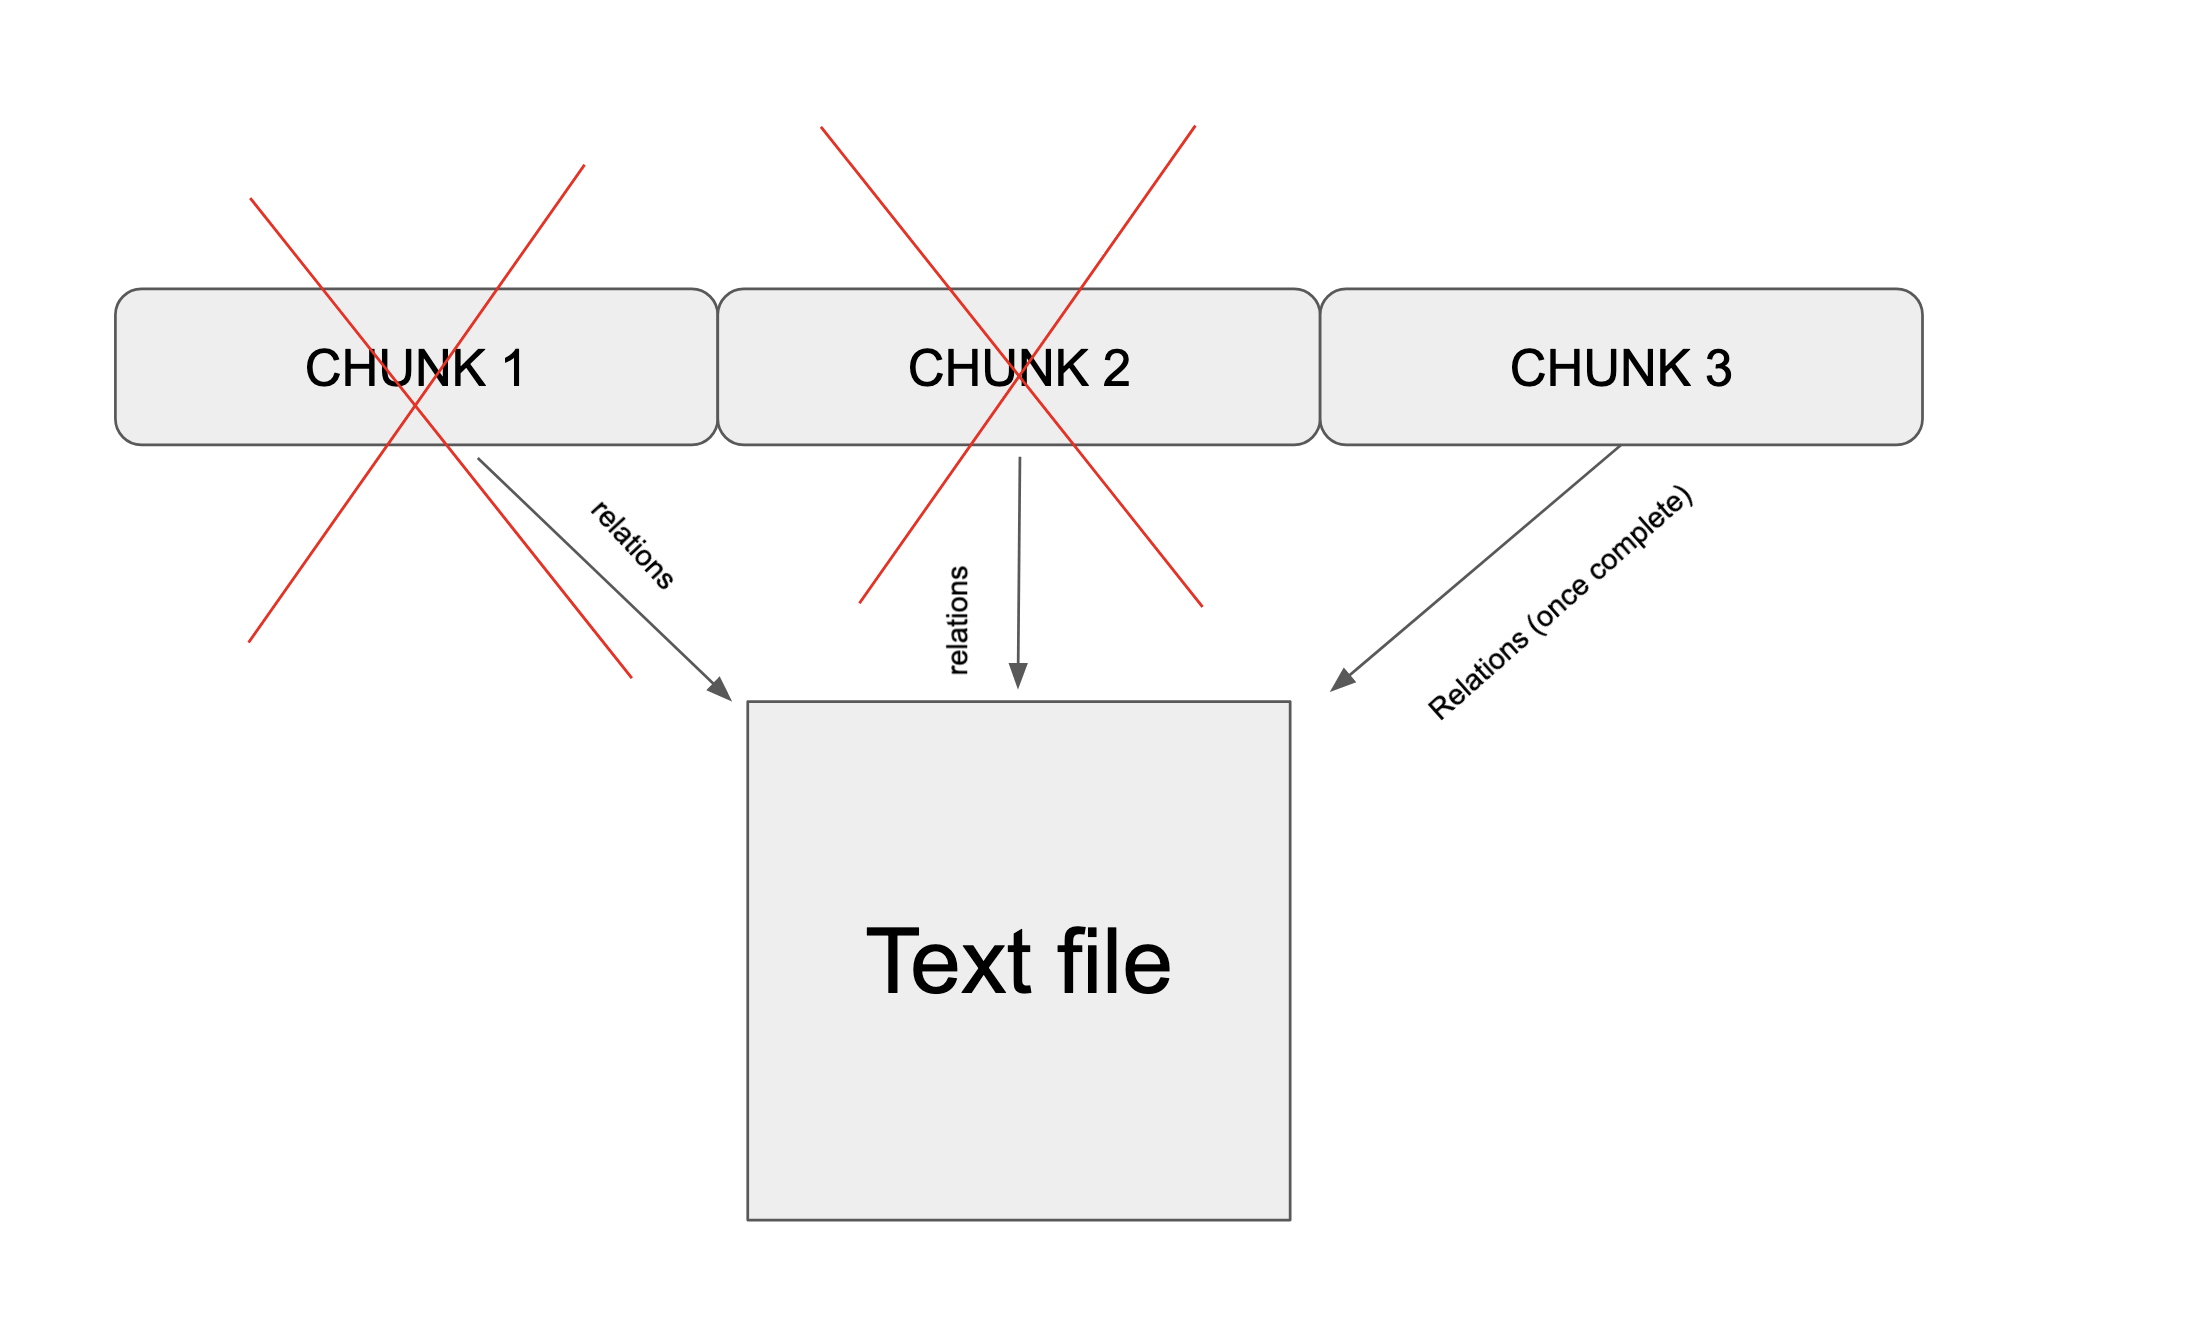
\includegraphics[scale = 0.2]{SieveSol.png}
    \caption{After writing relations from Chunk 1 and 2 and clearing those chunks from memory, we sieve chunk 3 and send relations once found}
    \label{Seq-Sieve}
\end{figure}

Once enough relations are gathered, we take what is carefully formatted and stored in the text file(s) and feed it into the linear algebra step. We then parallelized this in two ways. \\
\indent Our first MPI paradigm entails much communication between the boss and the workers. In particular, each worker creates and sieves through a designated chunk for all the relations and then sends them all to the boss. Note that we assign the chunks so that no two workers ever sieve over the same chunk, and each worker handles the memory for any chunk it creates. Then the boss sends the worker a message with information about whether to continue or stop sieving. If the worker is told to stop sieving, then it ends, and otherwise it sieves through the next designated chunk. Figure 3 shows how each worker is working on its own chunk and both sends and receives information from the boss.

\begin{figure}[!htb]
    \centering
   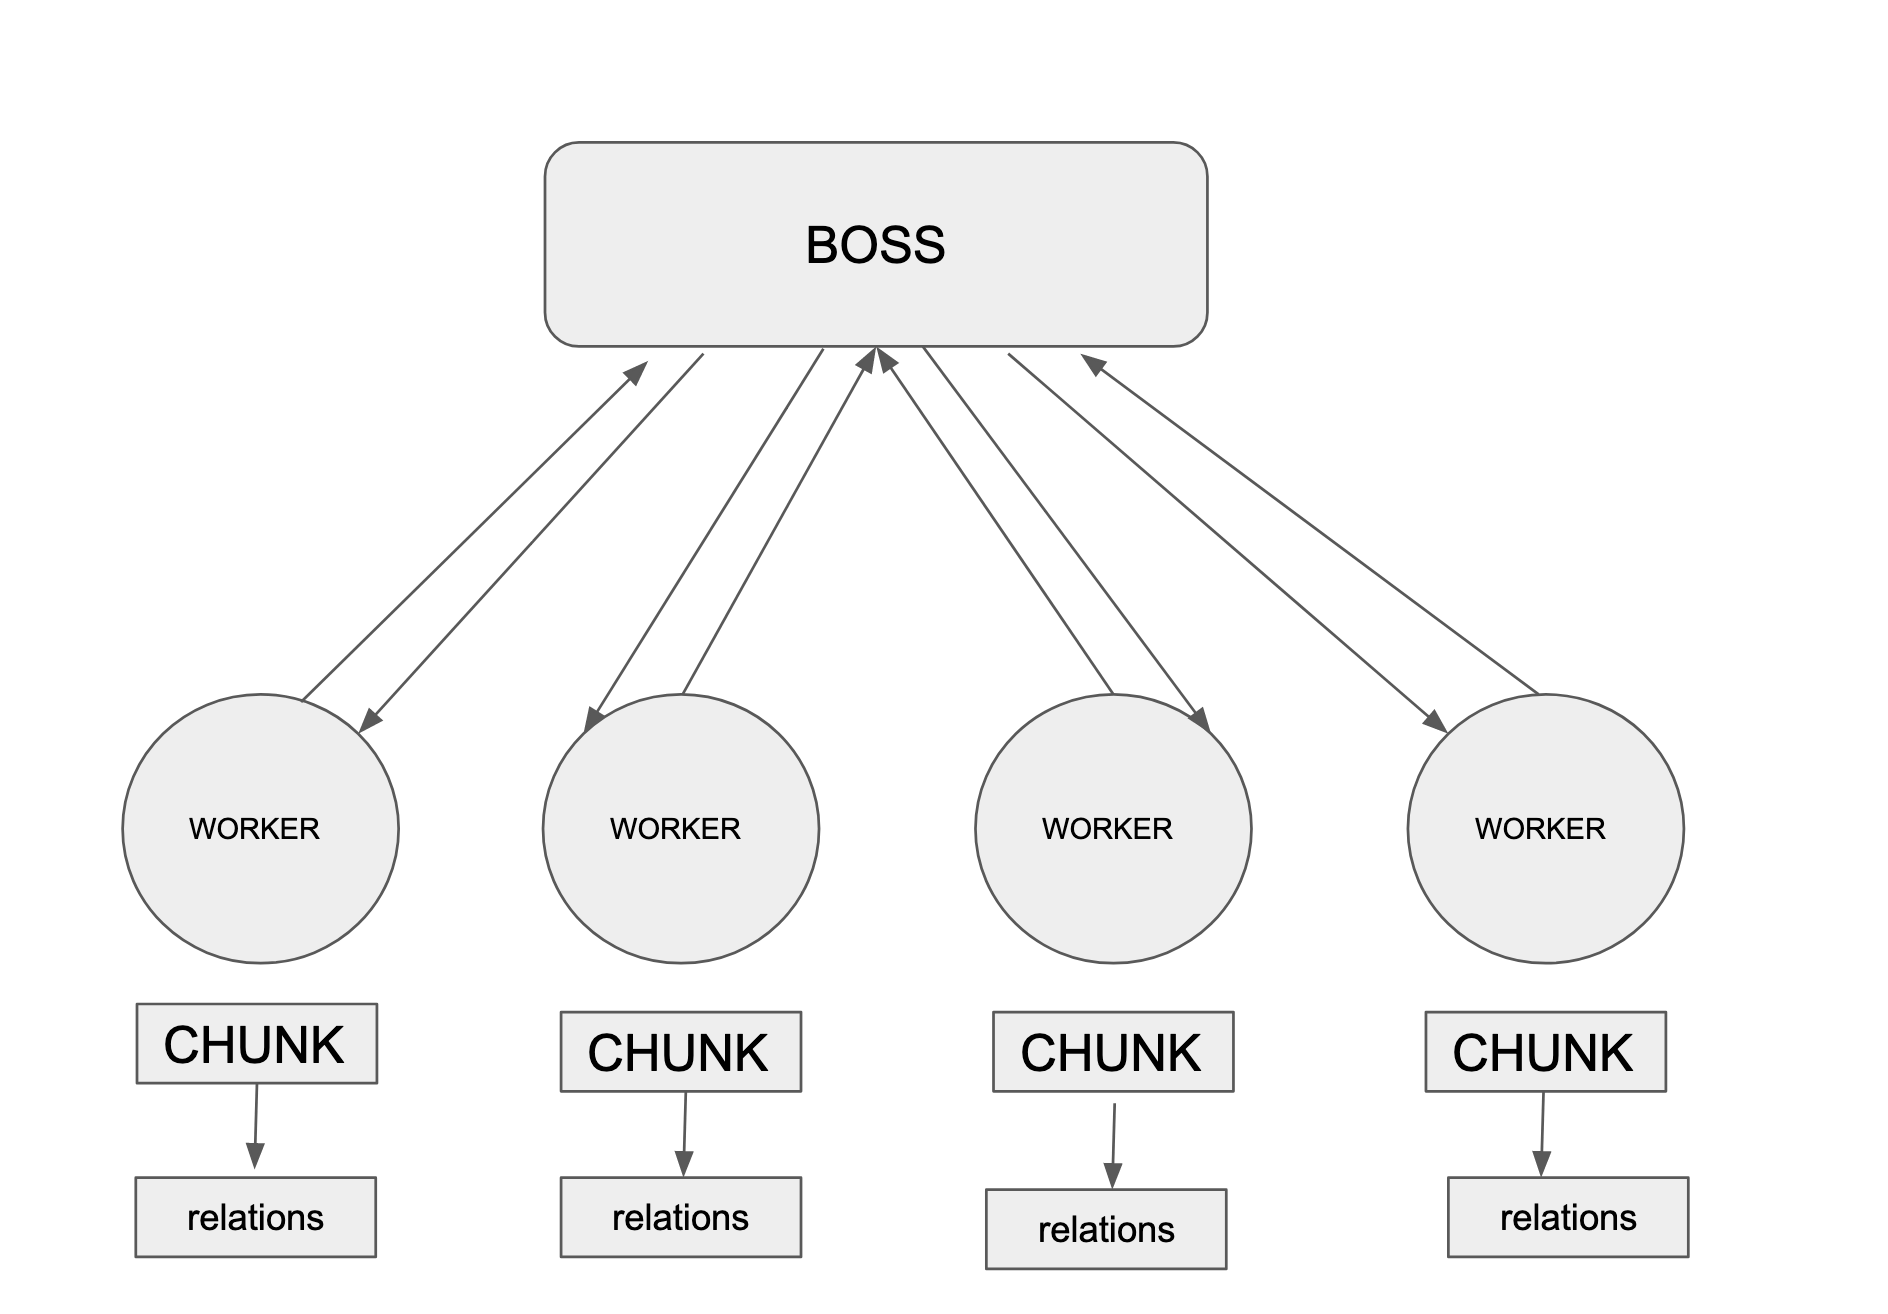
\includegraphics[scale = 0.2]{MPI-Para1.png}
    \caption{Each worker gathers relations from designated chunk before sending relations to boss and waiting for a response}
    \label{MPI-V1}
\end{figure}



For our second MPI paradigm, we have far less communication between the workers and the boss. In particular, each worker is told the amount of relations it needs to find. Then that worker continues to sieve through designated chunks, clearing the memory for chunks once it gets all the relations from them, until it finds the amount of relations that the boss needs. It then sends those relations to the boss, and the boss accepts them. Figure 4 depicts how workers clean their own memory while gathering enough relations for sending to the boss.

\begin{figure}[!htb]
    \centering
   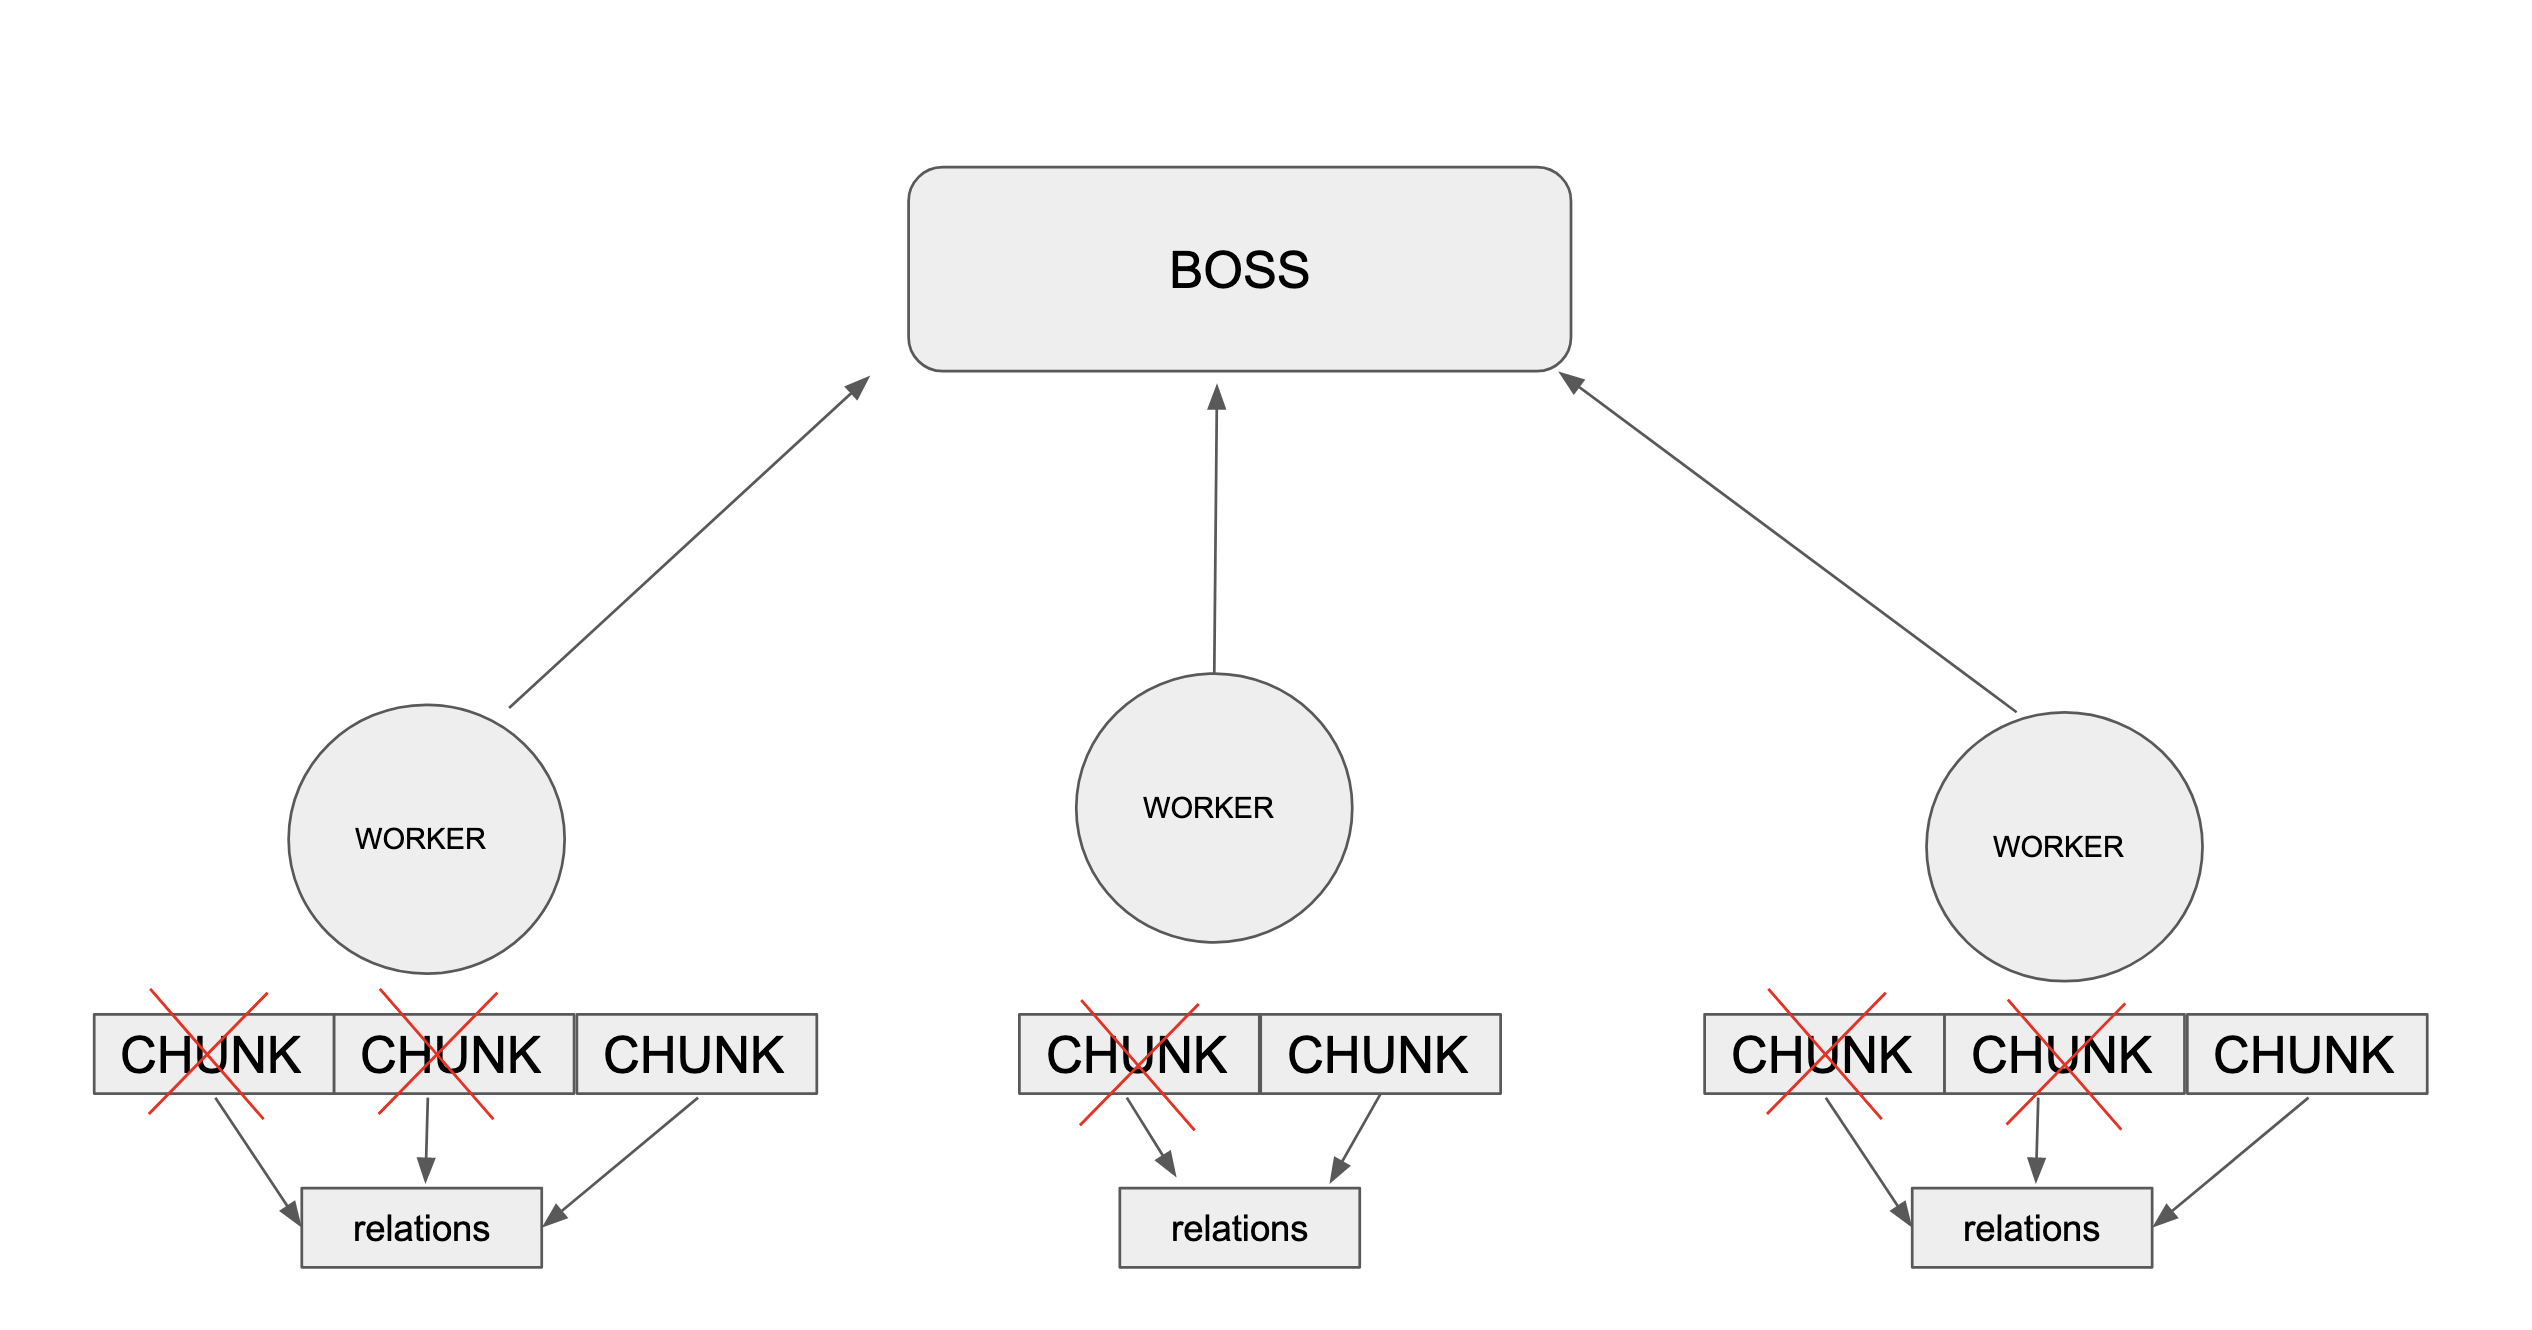
\includegraphics[scale = 0.2]{MPI-Para2.png}
    \caption{Each worker gathers relations from multiple chunks before sending relations to boss and clears older chunks from memory}
    \label{MPI-V2}
\end{figure}

\subsection{Results Overview}
We chose these two parallelizations because we do not know which might perform better. While the first parallelization requires more communication, it also allows a worker to make a larger contribution if it just happens to encounter more numbers which can be factorized over the factor base. On the other hand, the second doesn't allow this because it requires an equal contribution from each worker. Our experiments revealed that both parallelizations provide a massive speed-up. This makes sense because there is not communication needed among the nodes, and hence this is close to embarrassingly parallel. Furthermore, we find that for smaller keys, parallelization two is better. However, as the number of processes increases, parallelization one approaches parallelization two and in some cases performs better, given a large enough key size.



\section {Related Work}\label{relwork}
\indent While there have been multiple attempts to parallelize Quadratic sieve with MPI and CUDA, MPI is a markedly better fit for Quadratic Sieve because it is more difficult to handle large integers in CUDA. Furthermore, CUDA has far more space constraints due to GPU size while MPI can handle space constraints by simply adding more computers. Finally, copying such large values to the GPU is costly. Our literature review demonstrated the feasibility of using MPI as a parallelization tool and also gave some perspective on the GPU-compute power can be leveraged even with MPI.

\indent In 2000, Asbrink and Brynielsson \cite{asbrink:parallelqs} use a boss/worker model with MPI to parallelize sieving. Each node sieves designated intervals until it has accumulated a set amount of relations and then sends the relations to the boss node. The boss node either replies with a confirmation (in which case the node continues to sieve), or tells the node to terminate. The boss node then uses Gaussian elimination to find solutions, which are then tested to find a prime factor. Their paper describes that they implemented this method by having each of the nodes computing the factor base by themselves because all of them need it before sieving and also the boss node performs the Gaussian elimination; only the sieving step is done in parallel. In particular, the sieving interval is divided into some number of blocks, and the $i^{th}$ process sieves over the $i^{th}$ block so that all processes get a comparable distribution of large and small numbers. Once a node has found a designated number of relations, it uses a synchronized blocking send to the boss node. In response, the boss node tells the node to terminate if it has enough relations, and it sends the node a confirmation if needs more relations. Once the node starts using Gaussian elimination to find a solution from the other relations, the other nodes have to wait until Gaussian elimination is complete to receive termination. The authors note that the blocking sending/receiving can cause a worker node to be blocked unnecessarily and question whether a more decentralized approach could be better. The performance evaluation yields that using too many workers can lead to increased execution times due to the time spent initializing MPI.

\indent There is an available MPQS implementation that is based on the QS implementation in this paper \cite{bytopia:help}, and Papdoupoulous implemented an msieve library with tools which can be used to do steps or even all of MPQS \cite{papadopoulos:msieve}. In a paper for their implementation for MPQS \cite{jahenbaksh:mpiQS}, Jahanbaksh and Papadoupoulos describe more explicitly how the designated number of relations to be computed before sending should be a factor of how many relations are needed in total. While their implementation is for a multiple polynomial quadratic sieve, which divides the result of multiple polynomial implementations by primes and then groups relations for polynomials with a certain leading coefficient, it gives insight into how we may group blocks of relations in particular ways for our implementation.

\indent The papers by Asrbink and Brynnielson \cite{asbrink:parallelqs} as well as Papadapolous and Jahanbaksh \cite{jahenbaksh:mpiQS} gives a framework for how we can use MPI to parallelize step two of quadratic sieve by describing a specific boss/worker model which previously showed desirable speedup. Not only does it give us an immediate framework that we can implement, but it also points out some of the difficulties which we can address. In particular, it points  us towards further optimizing the boss/worker model and/or working around blocking behavior which has the potential to waste valuable CPU time. That provides some of the motivation for the MPI parallelisms that we used. These papers also give us a framework for how to measure speed-up with our sequential implementation measurements.

\indent A paper by Tordable  \cite{tordable:intmapreduce} introduces the MapReduce paradigm to the MPI parallelization framework. Tordable relates the QS algorithm with the MapReduce framework by describing the boss job as the \textit{controller} which generates the factor base and the interval which is to sieved and then splits the interval into pieces that are distributed to be sieved. The mapping step of the MapReduce framework corresponds to the sieving process, and the reducing corresponds to the linear algebra step. Tordable provides evaluation results which indicate that MapReduce may help with efficiency for medium sized problems. While a MapReduce framework might be a suitable way to reduce overhead, it does have initialization costs and this program does not have particularly complicated communication overhead. While its benefit may be somewhat ambiguous, the Map/Reduce framework opens the possibility of doing a distributed linear algebra solve without one node gathering all of the relations. Verma and Sharma \cite{verma:cudampilanczos} suggest a parallel Block-Lanczos solver for sparse linear systems which removes linearly dependent equations across nodes and then solves the remaining equations by using the broadcast function to share these dependencies. While this is an extensive project, this suggestion gives us a framework for how we could use CUDA-aware MPI to take advantage of the extra GPU compute power among the nodes for MPI.

\indent In addition to MPI parallelism, a project report by Pavan \cite{pavan:parallelgpu} describes the parallelization of pre-processing stages with CUDA, possible improvements, and the results. Pavan's implementation uses NVIDIA's CUDA to take advantage of the GPU's compute power. The algorithm implemented by Pavan uses the GPU to compute the factor base and implement Tonelli-Shanks algorithms. While Pavan found a 5x speed-up, it can be difficult to parallelize on GPU because polynomial arrays can become very large and then memory management will become too complicated. Archer and Wang \cite{archer:qsgpu} \cite{wang:qsgpu} were able to use GPU for the sieving step of the quadratic sieve. Archer details how it is possible to divide the interval into blocks since sieving step is independent for each of the numbers in the interval and describes various access patterns which can improve the efficiency of sieving. Wang also notes that it would be best to allocate subintervals which have size of the form $32k$ for $k \in \mathbf{N}$ because that will allow the GPU to coalesce data and save time that is spent accessing data from different locations, motivating our decisions for chunk sizes.

\indent While Pavan's pre-processing parallelization may sound appealing, much of the time it takes to run the algorithm occurs in the sieving step. Hence, as noted by Brynnielson and Asrbink \cite{asbrink:parallelqs}, it is best to direct our efforts towards parallelization of the sieving step. As we are performing the exact step multiple times on a single-dimensional array when we sieve, sieving is in large part a SIMD computation, and that is excellent for CUDA. As we are using a cluster of computers with GPUs, it is possible that CUDA can be used to benefit from that compute power.

\section {One or more sections describing your Solution}\label{soln}
We wrote our solution in C++ and used the GNU Multiple Precision (GMP) Arithmetic library, a library which allows us to handle large integers which cannot be stored in C++ datatypes. For our parallelization we used MPI. Even though MPI does not allow us to send mpz types from the GMP library, we were able to bypass this by storing and sending these large integers as strings. Our solution was mostly implemented on our own, but we used the MPQS solution published on Bytopia \cite{bytopia:help} as motivation for how to move between storing values as mpz types vs. int or long types, and we also took the Tonelli-Shanks algorithm verbatim from that implementation. While we would have liked to leverage the GPU-compute power, managing the interaction between large integers and CUDA is a much larger project.

\subsection{Sequential Implementation}
\indent We divided the sequential implementation into two parts. The first part generates the factor base and tells us how to identify for which $x$ we have that $p|Q(x)$ for some given $p$. While an approximation for the largest number in the factor base exists, in particular $B = (e^{\sqrt{ln(N)*ln(ln(N))}})^{\sqrt{2}}$ \cite{asbrink:parallelqs}, this is not something that we could compute with GMP. Furthermore, we found that practical implementations of Quadratic Sieve did not necessarily use a factor base this large. The author of the MPQS implementation we used \cite{bytopia:help} calculated a line of best fit with numbers noted by Silverman in a paper, but ultimately also used approximations conditioned on the amount of digits in $N$. We did something similar and used slightly larger numbers as we are implementing with a single polynomial. Our factor base may be sub-optimal from a mathematical perspective, but that isn't too consequential for our experiment. A small factor base requires less time per iterations, but it might require us to sieve through more numbers, and a large factor base has the opposite issue. However, quadratic sieve works regardless. As it is an inexact trade-off in either direction and both parallelizations are affected by it in the same way, it doesn't interfere with our results.

\indent After we determined the approximate size of the factor base, we used the approximation $2k \log(2k)$ \cite{archer:qsgpu} to find roughly the $k^{th}$ largest prime number. Then we used the Sieve of Eratosthenes, a mathematical method which is used to find all primes up to a number, to create the factor base of the approximate size. This was suggested by Asbrink and Brynnielson \cite{asbrink:parallelqs} as an alternative to using some library which finds the next prime. Recall that the purpose of our factor base is for these to be the primes which divide values of $x^2 - N$. For $p | (x^2 - N)$, we need $x^2 \equiv N \pmod{p}$. We use the \textit{legendre} function (from the GMP library) to check if this ever happens and remove all $p$ for which this is impossible. Then we also run the Tonelli-Shanks algorithm to find the two unique solutions $a$ and $b$ such that $a^2 \equiv b^2 \equiv N \pmod{p}$, because this tells us that $x^2 \equiv N \pmod{p} \iff x \equiv a, b \pmod{p}$. We save the size of the factor base and the values of the factor base (along with corresponding values $a$ and $b$) in a text file.
\indent We can now enter step 2, which is the sieving step. We start by creating a chunk of size 16,000 which corresponds to the set $\{Q(x) | x \in [T, T + 16000) \}$, where $T = \lfloor \sqrt{N} \rfloor + 1$ and $Q(x) = x^2 - N$. Then for each prime $p$, we find the smallest $Q(x)$ in that chunk such that $x \equiv a \pmod{p}$. Then $Q(x)$ is divisible by $p$ and then so is $Q(x + kp)$ for any $k \in \mathbf{N}$. Thus, we go through the chunk and divide each $Q(x + kp)$ by $p$ as many times as possible. We repeat the same process for the smallest $Q(x)$ such that $x \equiv b \pmod{p}$. Then we go to the next prime and continue. In Figure 5, let the arrow labeled with smallest val point to the smallest location where $Q(x)$ was evaluated on some $x \equiv b \pmod{7}$. Then we can repeatedly add $p = 7$ to find all the other locations where this holds

\begin{figure}[!htb]
    \centering
   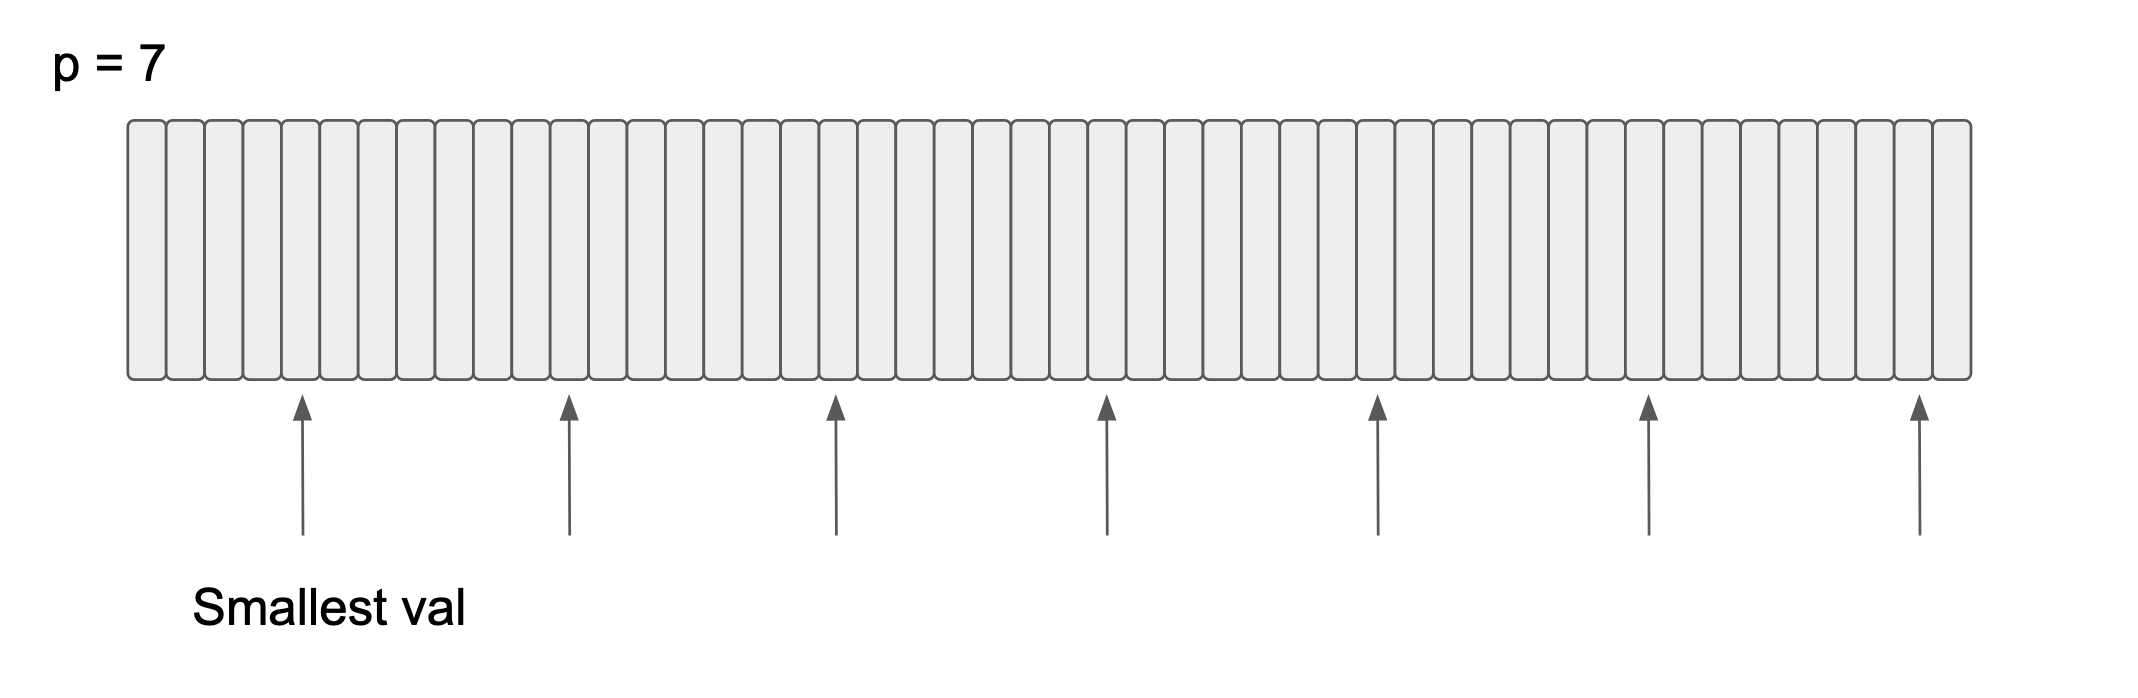
\includegraphics[scale = 0.2]{Tonnelli.png}
    \caption{Upon finding smallest evaluation divisible by $p$, arrows point to what else we know is divisible}
    \label{Tonnelli}
\end{figure}

While we do this, we are keeping track of (1) the total amount of relations found by counting if some $Q(x)$ got divided down to 1 (2) what primes each $Q(x)$ has been divided by and how many times, and (3) which $Q(x)$ have been divided down to 1. We keep track of (2) and (3) with a matrix like this: \\

$\begin{pmatrix}
e_{1, 1} & e_{1, 2} & e_{1, 3} & \cdots & e_{1, m} \\
e_{2, 1} & e_{2, 2} & \cdots & & \\
e_{3, 1} & \vdots & \ddots & & \vdots\\
\vdots & & & & \\
e_{n, 1} & & \cdots & & e_{n, m} \\
b_1 & b_2 & \cdots & & b_m
\end{pmatrix}$


We initialize all values in this matrix to $0$. If we find that $p_i$ divides $x_k^2 - N$ perhaps $3$ times during the sieving step, then we set $e_{i, k} = 3$. The last row is also initialized and set to $0$ and changing $b_k$ to $1$ indicates that $x_k^2 - N$ has been fully factored. In total, we are looking for $B + 10$ relations, where $B$ is the size of the factor base. If at any time our counter exceeds $B+10$, we stop sieving immediately and gather our relations. Otherwise, we wait until the interval has been sieved with all the primes in our factor base. Once we finish sieving, we gather fully factored relations and write them into a file. In particular, each line in our file is the powers of a factorization. This is achieved by finding the columns with $b_k = 1$ and then making all the values above it into row(s), as shown in Figure 6.  \\

\begin{figure}[!htb]
    \centering
   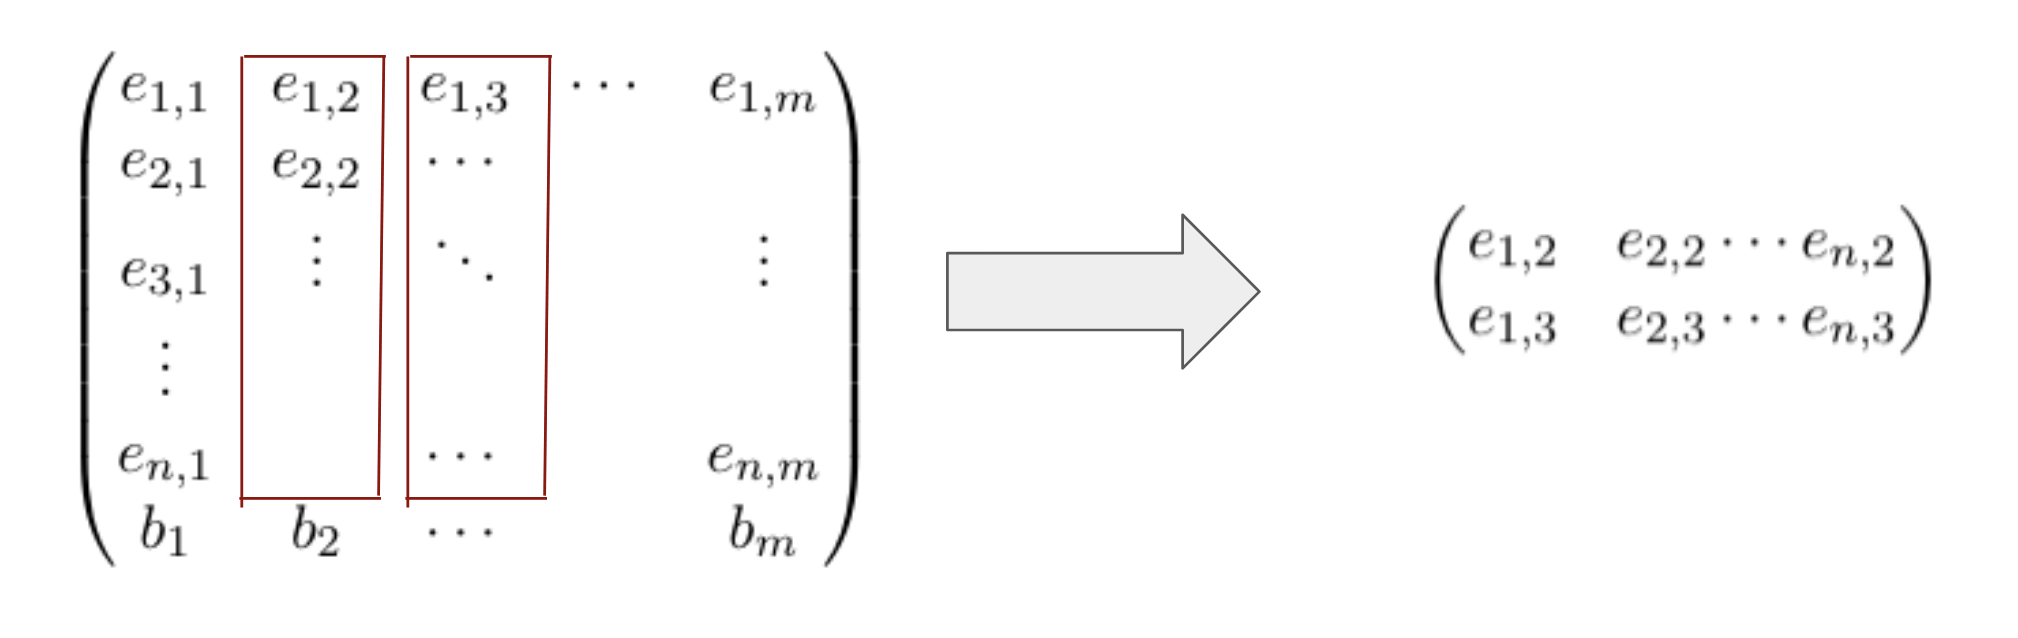
\includegraphics[scale = 0.2]{fileread.png}
    \caption{Finding columns which have all the information needed to factor the number, we write it as row(s) into a text file}
    \label{Tonnelli}
\end{figure}



Likewise, we gather all the values of the $x_k^2 - N$ which were successfully factored into another text file in the same order. We also generate a bit matrix which is all $e_{i, j} \pmod{2}$. This is just done by taking mod 2 of all the elements in the other matrix. Now if we found enough relations, we are done. If not, we generate the next chunk and repeat the same step. All the while, a counter is keeping of track of all the relations we have found since the first chunk, and so sieving on a chunk terminates as soon as enough relations are found. Note in general that we'll be sieving over the set $\{Q(x) | x \in [T + (m-1)16000, T + (m)16000 \}$ during the $m^{th}$ iteration. \\
\indent In an ideal world, we would then solve the equation. However, we could not find any C++ libraries which would allow us to find several solutions and spent a ridiculous amount of time on this part. We found someone's Python implementation, but they generated the factor base differently from us. Ultimately, we decided to exclude the final step here and focus on the parallelization to achieve what we wanted: parallelize quadratic sieve. However, the addition of a solver would be very nice as it will allow us to see the final factorization.

\subsection{MPI Implementations}
For both MPI implementations, we designate the chunks of the sieving interval to processes cyclically. This ensures that all processes are dealing with similarly sized chunks so that the load is distributed more evenly. For example, if there are 3 worker processes, then the first one can get the white processes, the second the gray, and the third the black, and the distribution is what is shown in Figure 7.

\begin{figure}[!htb]
    \centering
    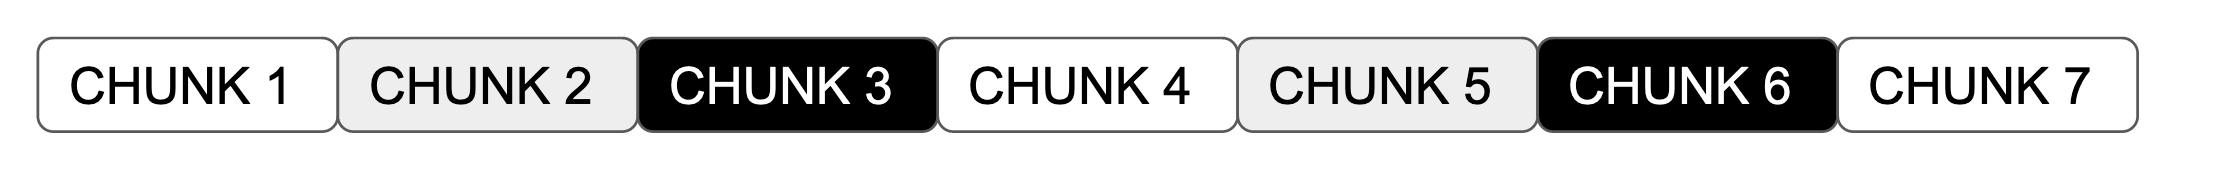
\includegraphics[scale = 0.2]{chunks.png}
    \caption{Distribution of chunks among 3 nodes}
    \label{chunks}
\end{figure}

Just because a chunk is designated for a process doesn't mean that the process will reach that chunk. If it's task ends earlier, or if the boss tells it to stop, then the worker will never generate that chunk. It follows from arithmetic here that the $i^{th}$ worker sieves over the chunk $\{Q(x) | x \in [T + (i-1) \cdot 16000 + 16000(nm),  T + i \cdot 16000 + 16000(nm) \}$ when there are $m$ workers and on the $(n+1)-st$ iteration, and we enable this by carefully generating the sieving interval from the lower bound of this set during the appropriate iteration. \\
\indent For our first MPI implementation, each worker sieves over its current designated chunk. It gathers the factorizations into a 2D array with rows similar to as described earlier and all of the numbers which were factorized into an array. It then sends the number of gathered factorizations to the boss with MPI-Send(). The boss uses MPI-Recv() to receive from any node. Once it receives an integer number from any worker, it then receives only from that worker until all the information is received. The boss then uses MPI-Recv() to receive the next three MPI-Send() from that worker. These sends are a contiguous 2D array with all the factorizations, the length of an array of characters which contains all of the factorized numbers mashed together, and then the array of characters. The boss takes all of the relations or as many relations as needed to have $B+10$ relations and writes them to file(this can be none if the boss already has enough from others). Then it uses MPI-Send() to tell the worker whether or not it should continue to work. The worker then uses MPI-Recv() to get this information and either terminates or continues to sieve. Even though the worker cannot know if it is producing too many relations since it doesn't have the information the boss does, we do have the worker stop sieving and send relations if it has generated more than $B+10$ relations itself through all the chunks so far. \\
\indent For our second MPI implementation, the worker does exactly the same job with each chunk. However, instead of sending it to the boss, the worker has a 2D array of fixed size to store all of the relations extracted from each chunk and also a 1D array of fixed size to store all the numbers that can be factored. It continues to sieve chunk by chunk until these arrays are filled and deletes each chunk after extracting the necessary information from it. Figure 8 shows how these additional relations are stored geometrically with respect to the previous relations.

\begin{figure}[!htb]
    \centering
    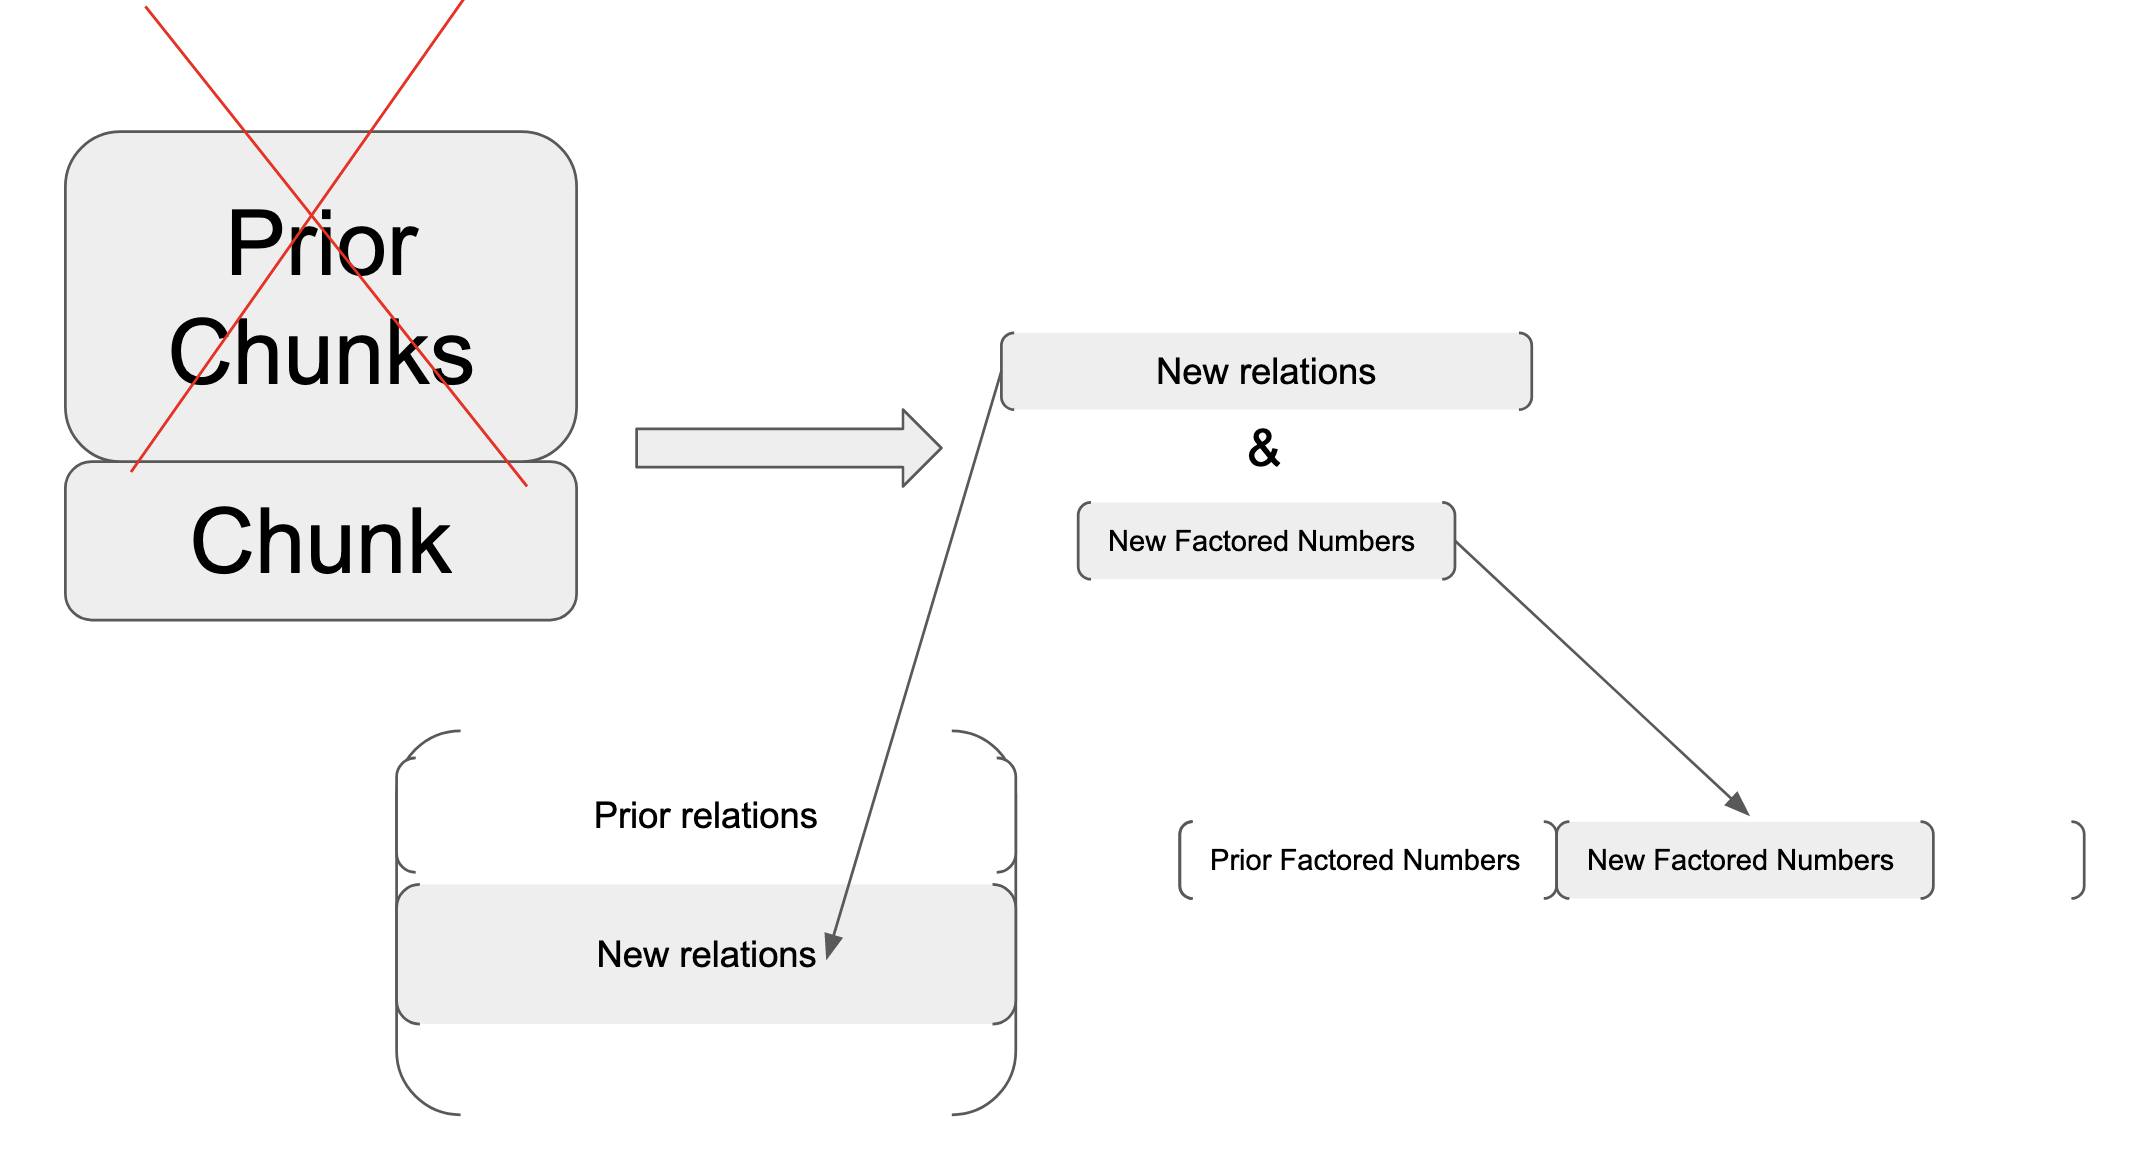
\includegraphics[scale = 0.2]{Para2Chunk.png}
    \caption{After finding relations from a chunk, process adds relations to previously gathered relations from previous chunks, all of which have been cleaned}
    \label{chunks}
\end{figure}


There is a running counter which keeps track of many relations have been found in total thus far, and the algorithm immediately stops sieving after it finds the amount of relations which have been designated to it. Once these arrays are full, the worker sends the number of gathered factorizations to the boss with MPI-Send(). The boss uses MPI-Recv() to receive from any node. Then the message passing protocol is the same as the first implementation. The boss writes the relations and numbers to file, and this continues until it has received relations from all the workers.


\section {Results}\label{results}
We performed sieving over a variety of key sizes over four iterations and recorded the average time. The key sizes which were most relevant for us were 20 digits, 30 digits, and 38 digits. While Asrbink and Brynielsson \cite{asbrink:parallelqs} tested keys that were between 45 and 60 digits, this was (a) not feasible for our testing environment, which is the Swarthmore cluster system and (b) not feasible to perform with multiple iterations due to the long runtime, which was further exacerbated because we used division instead of log subtraction. These tests were performed using MPI on Swarthmore computers during times with less computer usage, such as Sunday afternoon and during the night.

\begin{figure}[!htb]
    \centering
    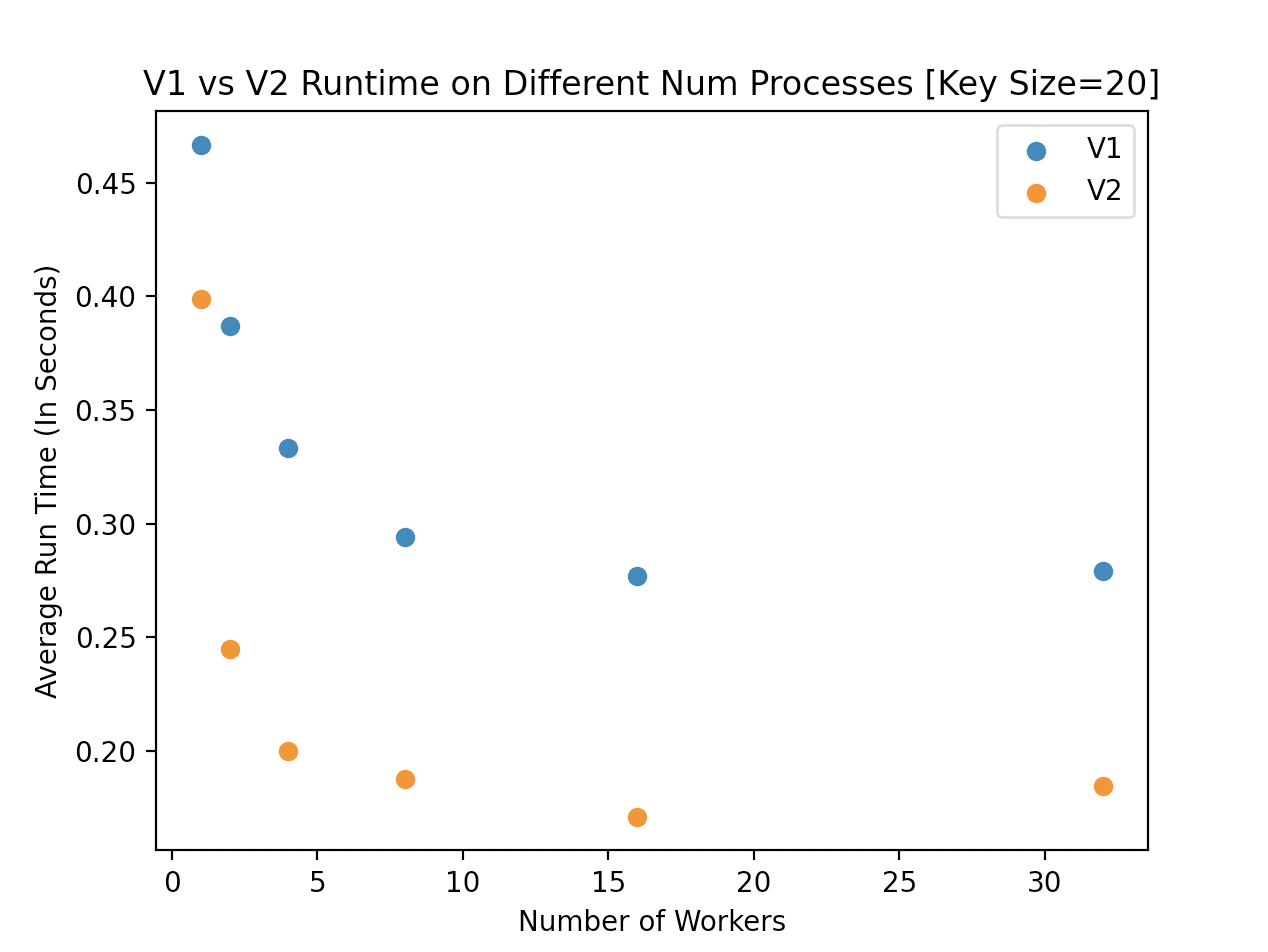
\includegraphics[scale = 0.2]{20.png}
    \caption{20-digit key runs}
    \label{20dig}
\end{figure}

\begin{figure}[!htb]
    \centering
    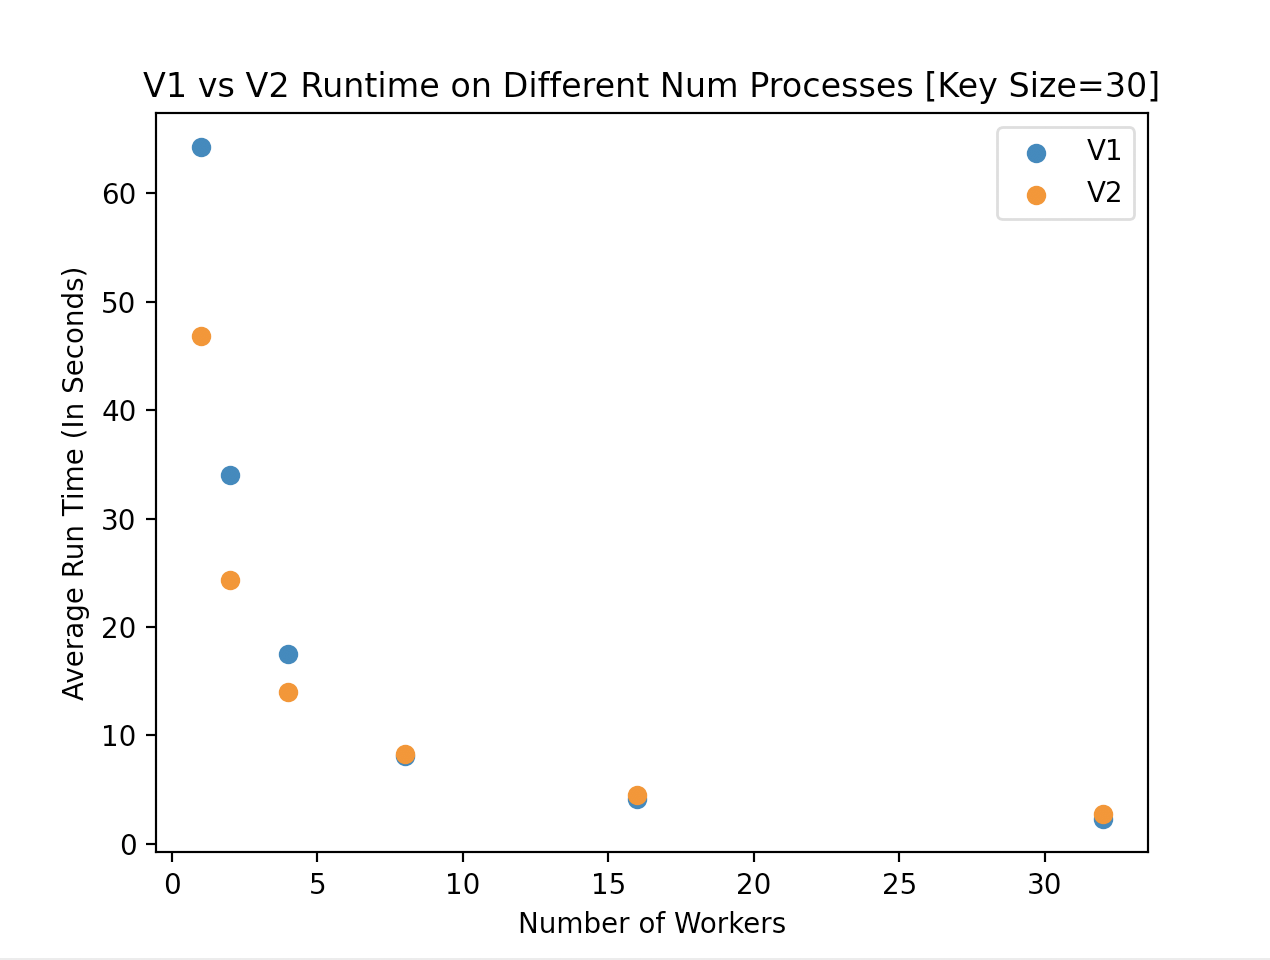
\includegraphics[scale = 0.2]{30.png}
    \caption{30-digit key runs}
    \label{30dig}
\end{figure}

\begin{figure}[!htb]
    \centering
    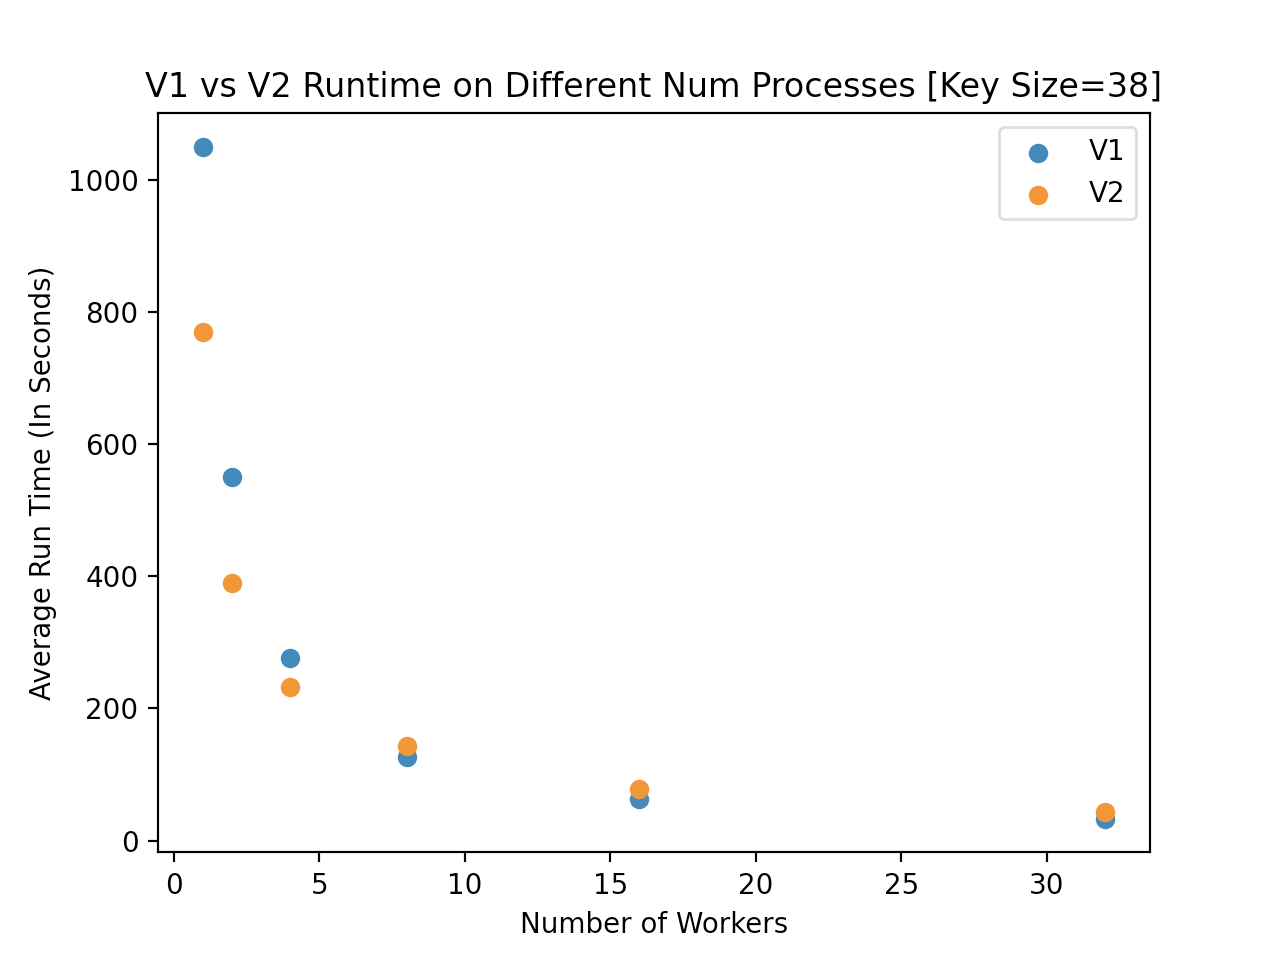
\includegraphics[scale = 0.2]{38.png}
    \caption{38-digit key runs}
    \label{38dig}
\end{figure}

The results, in this scope of testing, are consistent with our initial intuition: for smaller key sizes and smaller amounts of worker processes allocated, the first MPI implementation of our sieving step (V1 hereafter), performs worse than the second MPI implementation of our sieving step (V2 hereafter). Because V1 has significantly more communication overhead than V2, it is likely to perform worse on smaller key sizes - simply put, V1 spending that extra time communicating back and forth takes up more time than V2's approach to having the workers waste no time communicating and just sieve. Furthermore for small keys, the advantage from having some worker nodes contributing more than others is minimal (V1 worker nodes have no upper bound on how many relations they are allowed to contribute, whereas V2 worker nodes do have an upper bound).\\
\indent However, for larger key sizes, given a sufficient amount of worker nodes allocated, this communication overhead present in V1 proves to be useful. Though slight, as seen in figures 10 and 11, the average run time of our sieving step in V1 is better than V2 (after eight nodes). An intuitive reason for this improvement in run time is as follows: for big key sizes it is really important that certain worker nodes are able to contribute more than others. For example, in V1, if worker node A is able to compute relations much faster than its peers, the boss node has the ability to tell node A to continue sieving (taking advantage of its speed). Whereas in V2, even if worker node A is able to compute relations much faster than its peers, it must still abide by its given upper bound and stop sieving for relations when it has met its goal - thus the whole system would not be able to utilize node A's faster speed.\\
\indent It should also be noted that, even for larger key sizes, V1 is still slower than V2 when we use smaller amounts of worker nodes (more specifically less than eight nodes in this case). Again, the key strength in V1 is its ability to take advantage of the discrepancies in the different worker nodes' performance (a fast worker node can make up for other worker nodes' comparatively poorer performance). A smaller amount of worker nodes means there is likely to be less variance in the performance among the worker nodes. But with a larger amount of worker nodes, there is likely to be more variation in worker node performance. Thus, by using more worker nodes, V1 is better able to exploit this variance.

\begin{figure}[!htb]
    \centering
    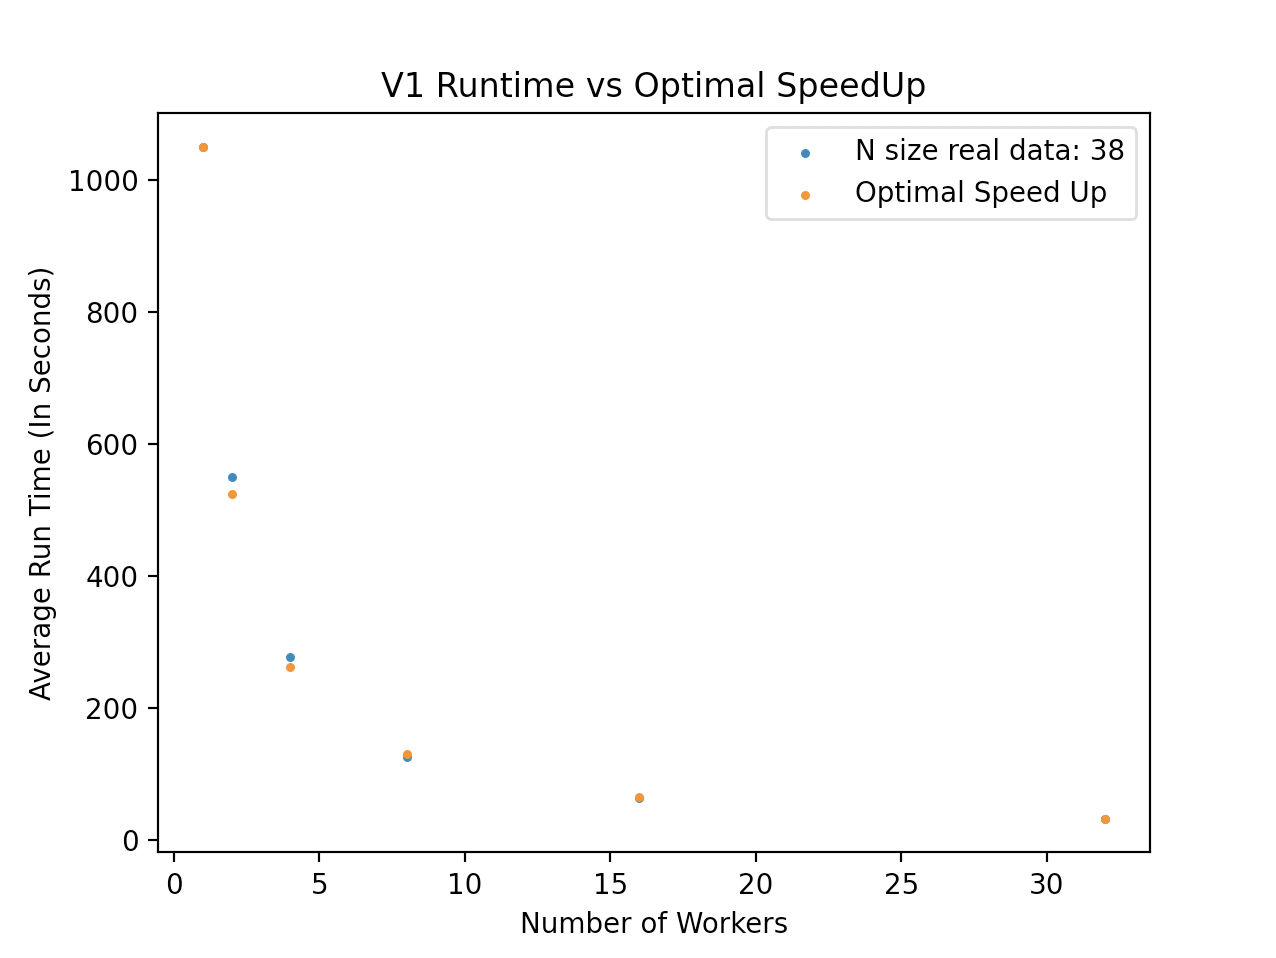
\includegraphics[scale = 0.2]{V1-speedup.png}
    \caption{Results vs. Optimal Speedup Results}
    \label{V1-speedup}
\end{figure}


\begin{figure}[!htb]
    \centering
    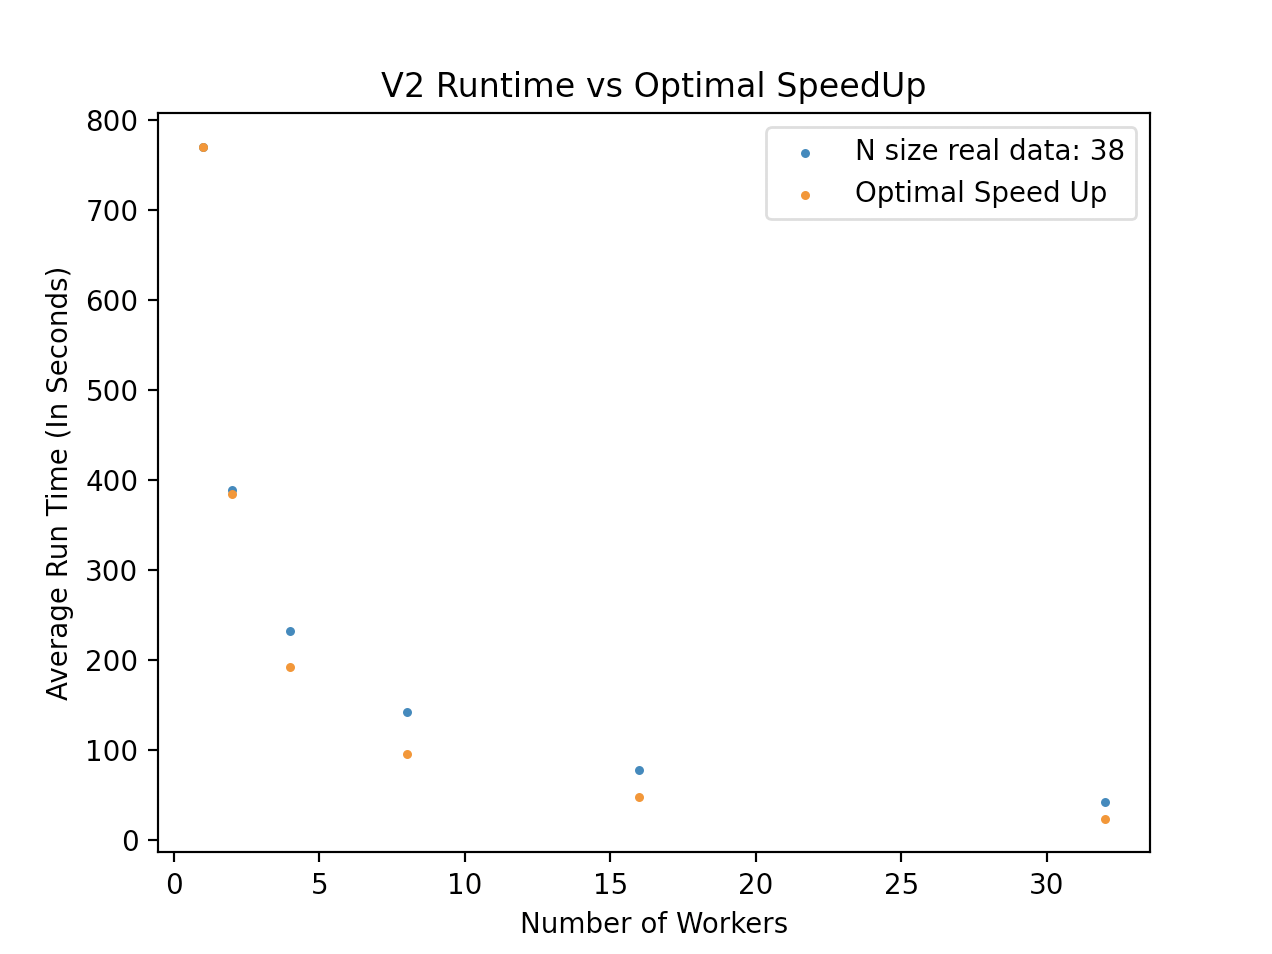
\includegraphics[scale = 0.2]{V2-speedup.png}
    \caption{Results vs. Optimal Speedup Results}
    \label{V2-speedup}
\end{figure}

\indent It is worth noting that both V1 and V2 were able to achieve close to optimal speed up (note: we determined optimal speed up by taking the run time of one worker node and dividing the run time in half each time we double the amount of worker nodes, for both figure 12 and figure 13). V1 is gets much closer to the desired optimal speed up, with deviations in mid sized amounts of worker nodes. This further corroborates the point that the ability to exploit the variance in worker nodes performance is much more potent as the number of worker nodes increase. With this in mind, with little overhead communication, V2 was not able to achieve as close to optimal speed up as V1 was able to, and we think this is because V2 did not have the communication protocols to help optimize its speed up.


\section{Conclusions and Future Directions}\label{conc}
Our work demonstrated to us that embarrassingly parallel strategies lead to significant speedup and also indicate that increased communication to allow for more flexibility in worker contribution can be helpful for larger keys and with more nodes. We are interested in how well our observations hold up for real-world large-sized keys and a larger number of processes, and this is a potential future direction. Furthermore, we are interested in seeing how much our MPI parallelization would be improved by adding a CUDA component. While CUDA can definitely make our sieving process faster, it is costly to copy data into the GPU, and we are interested in seeing whether it is worth it. Finally, it is also possible to parallelize the third step in conjunction with the second using MapReduce, and we are interested in how much better it would be than just parallelizing the second and third step separately.





\section{Meta-discussion}\label{meta}
Everything was difficult. The theoretical portion of this project alone combines multiple upper level disciplines, including but not limited to, number theory, cryptography, linear algebra, and probability. Even though we focused on just a few specific aspects of the Quadratic Sieve, it was difficult to implement the theory into code.\\
\indent This difficulty in implementation is due to several reasons. First, we are dealing with extremely large numbers, which standard low level languages are not able to handle without the help of outside packages (for this project we used the GMP library to handle large multi-precision numbers). Second, though these packages have helped, they also brought a host of issues as well. An example is the difficulty in memory management and data structure design, as certain aspects of these packages do not behave as we would expect a standard datatype would. Furthermore, it is much more difficult to debug GMP library types with GDB. Another example of the difficulty that the GMP libraries have brought is their limited range of arithmetic operations that they were able to perform - thus we had to get creative to fit our implementation to the outlined theory as best as we could. A last example of the difficulty is the incompatibility of GMP with parallel languages, especially CUDA, forcing us to abandon the CUDA portion of our project given the time constraints - it should be noted that it does not work well with MPI either, but we were able to handle it by converting GMP types into char arrays to send and receive. \\
\indent While we had hoped that we would incorporate CUDA into MPI, we decided to have 2 MPI parallelizations. We had also earlier thought that we would use Map Reduce as one of our MPI parallelizations, but we decided against that because it didn't seem to bring much advantage unless we were also doing step 3 in parallel.





% The References section is auto generated by specifying the .bib file
% containing bibtex entries, and the style I want to use (plain)
% compiling with latex, bibtex, latex, latex, will populate this
% section with all references from the .bib file that I cite in this paper
% and will set the citations in the prose to the numbered entry here
\bibliography{finalreport}
\bibliographystyle{plain}

% force a page break
\newpage
% I want the Appendices to be single column pages
\onecolumn
\section{Appendices}\label{appx}

We include other graphs that we did not include in our paper.



\begin{figure}[!htb]
    \centering
    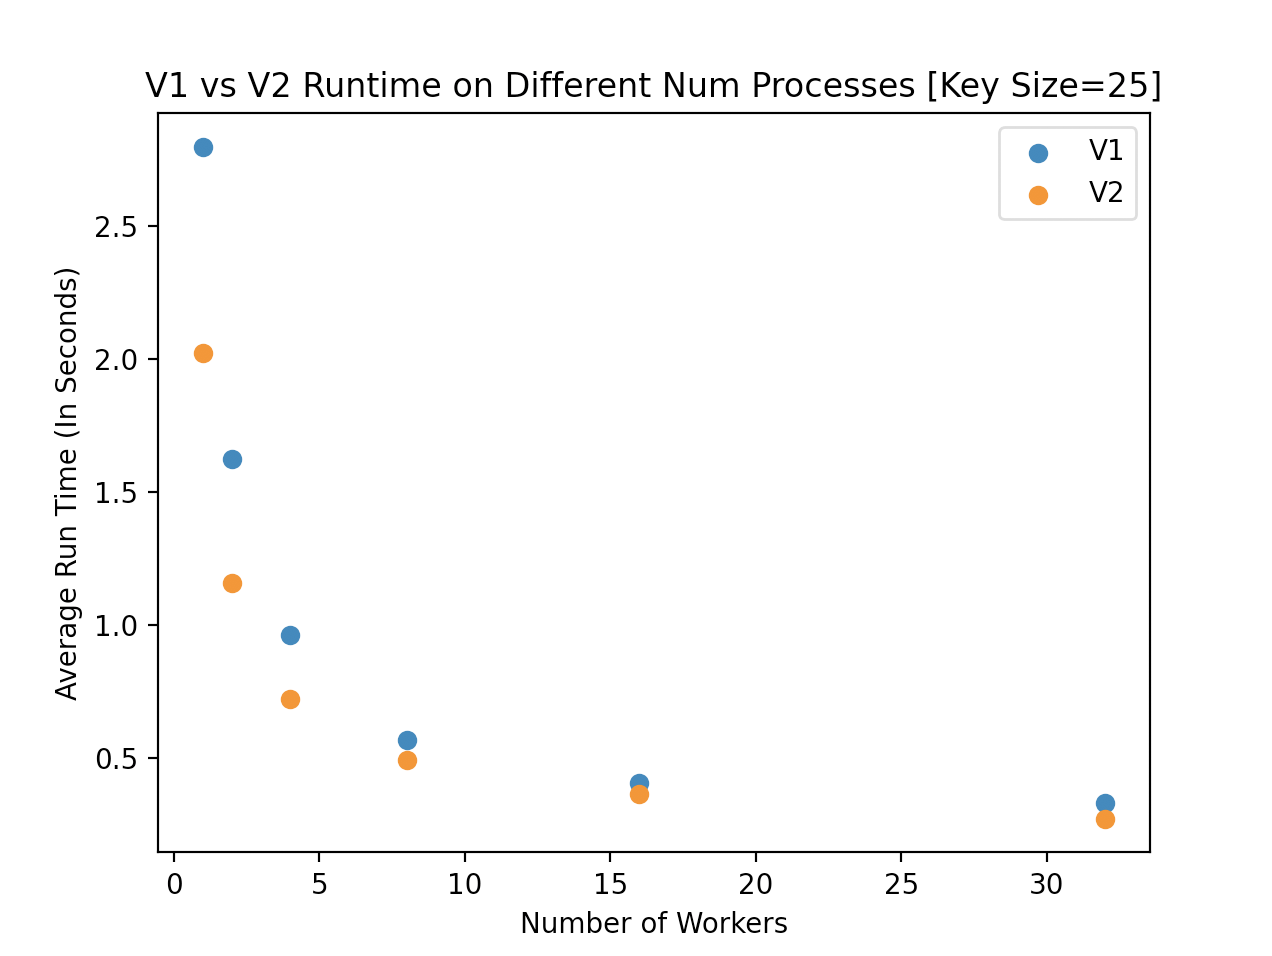
\includegraphics[scale = 0.2]{25.png}
    \caption{Results for key size 25}
    \label{V2-speedup}
\end{figure}

\begin{figure}[!htb]
    \centering
    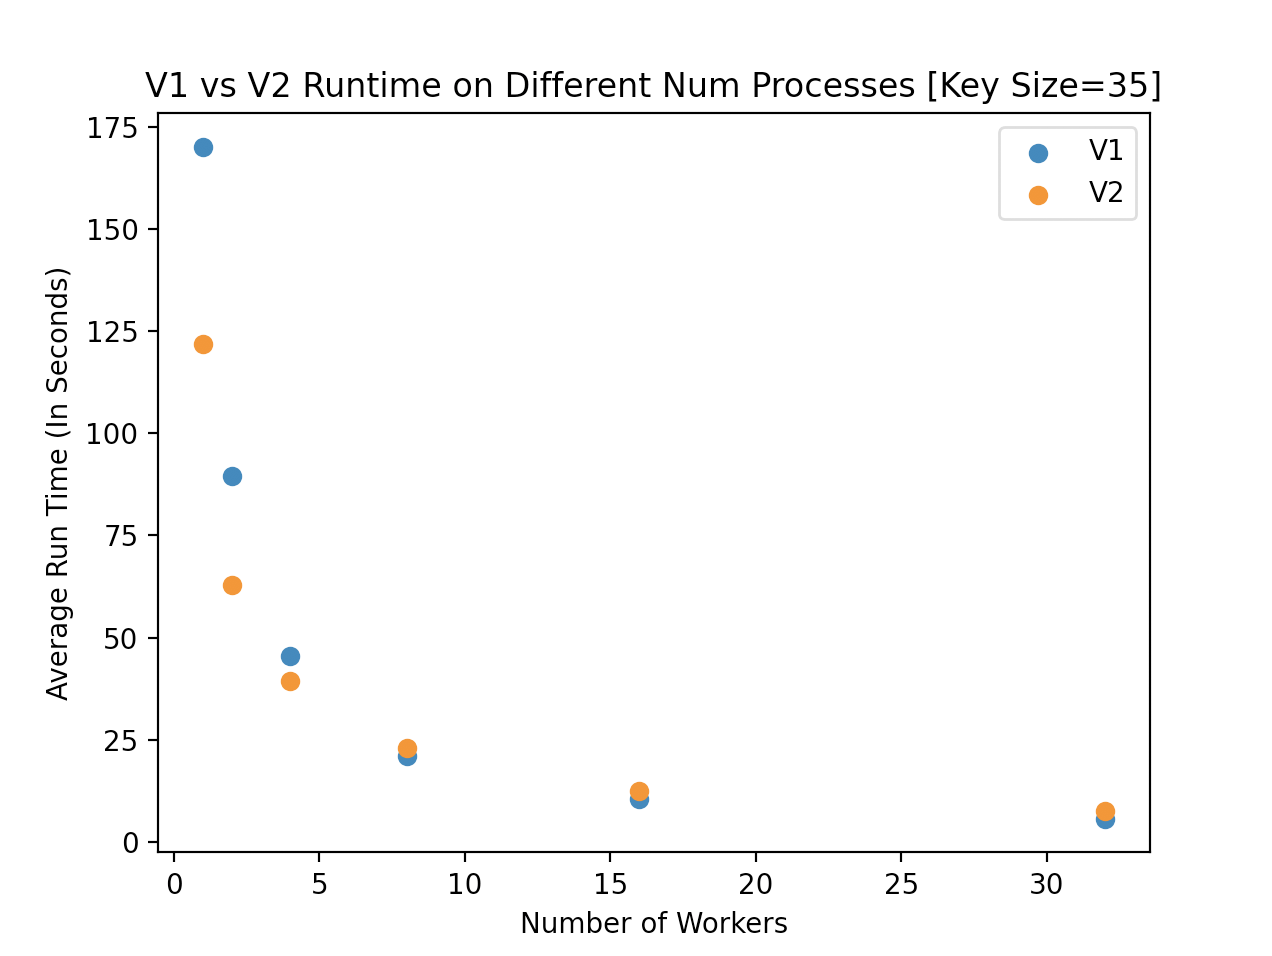
\includegraphics[scale = 0.2]{35.png}
    \caption{Results for key size 35}
    \label{V2-speedup}
\end{figure}


\begin{figure}[!htb]
    \centering
    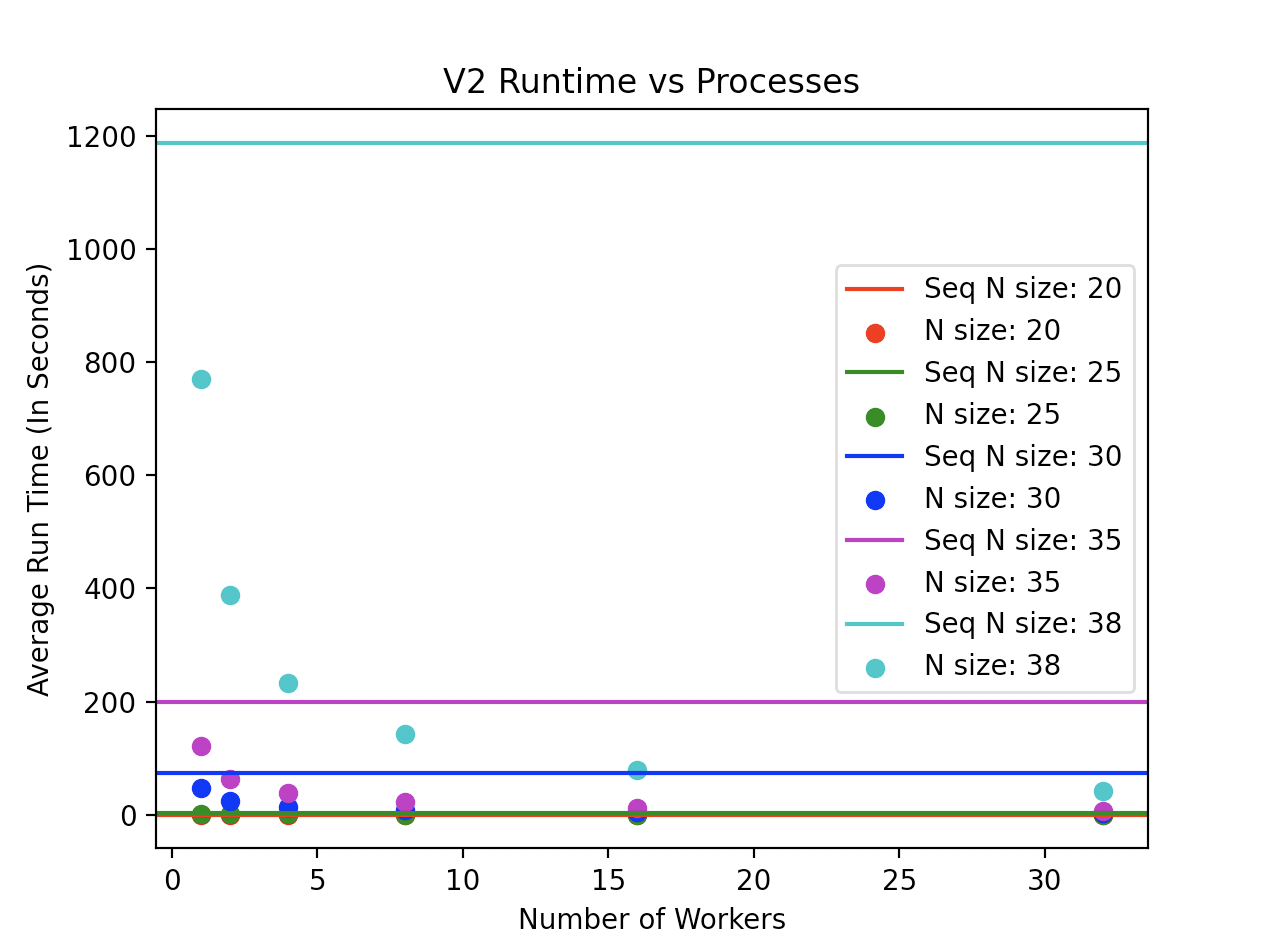
\includegraphics[scale = 0.2]{V1ALL.png}
    \caption{All results for V1}
    \label{V2-speedup}
\end{figure}


\begin{figure}[!htb]
    \centering
    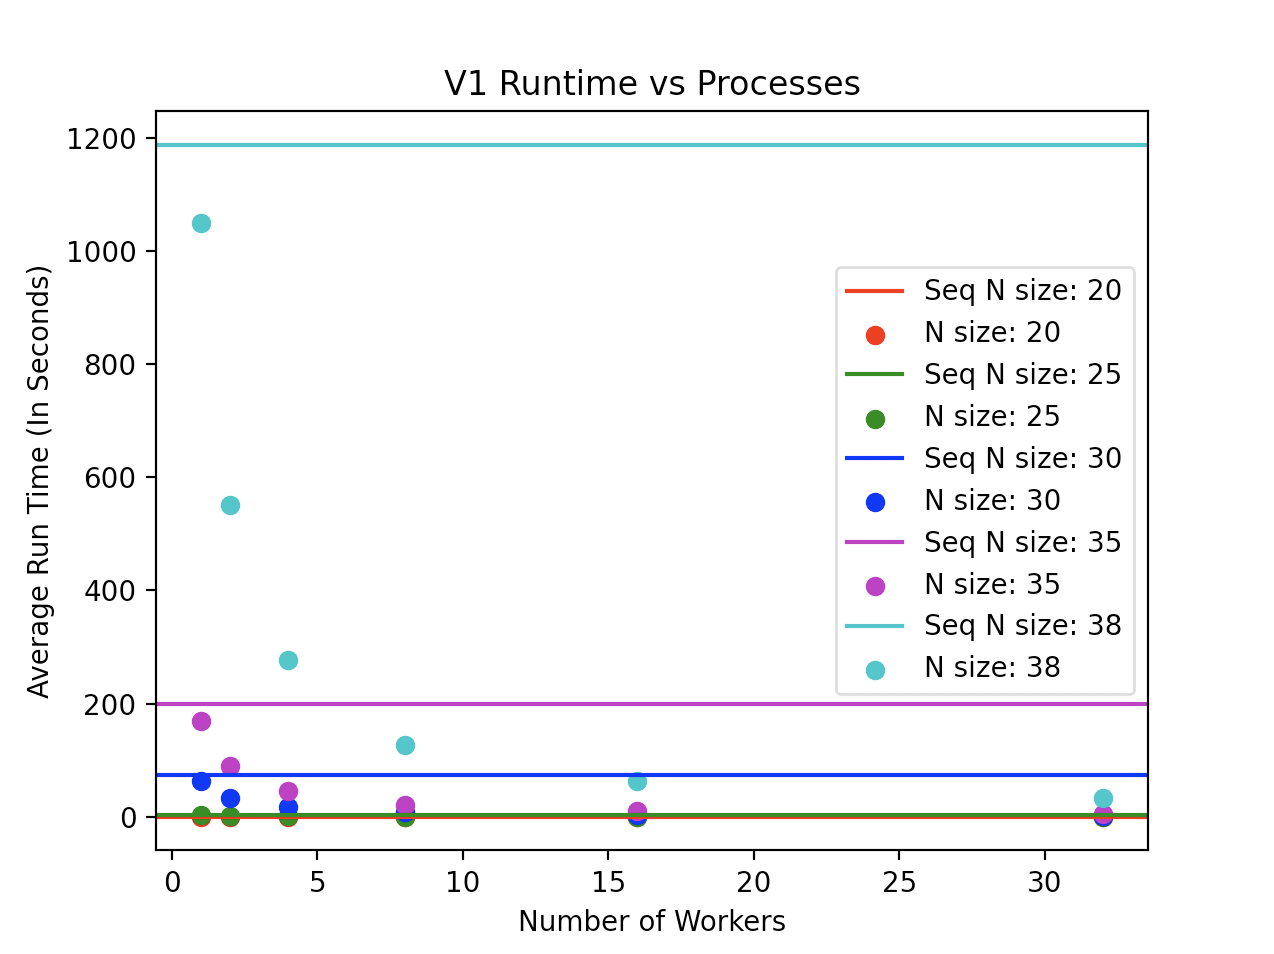
\includegraphics[scale = 0.2]{V2ALL.png}
    \caption{All results for V2}
    \label{V2-speedup}
\end{figure}

\end{document}
